\documentclass[wevj,article,submit,moreauthors]{Definitions/mdpi}
\def\rootdirectory{/home/dmortensen/paper1/MILP_planning_paper/paper}
\def\builddirectory{/home/dmortensen/paper1/MILP_planning_paper/paper}

\usepackage{amsmath,amsfonts}
\usepackage{array}
\usepackage{textcomp}
\usepackage{tikz}
\usetikzlibrary{positioning}
\usetikzlibrary{math}
\usetikzlibrary{shapes}
\usepackage{pgfplots}
\usepackage{pgfplotstable}
\pgfplotsset{compat=1.7}
\usepgfplotslibrary{dateplot}
\setcounter{MaxMatrixCols}{20}
\usepackage{subfig}
\usepackage{stfloats}
\usepackage{url}
\usepackage{verbatim}
\usepackage{graphicx}
\usepackage{mathtools}
\hyphenation{op-tical net-works semi-conduc-tor IEEE-Xplore}
\def\BibTeX{{\rm B\kern-.05em{\sc i\kern-.025em b}\kern-.08em
    T\kern-.1667em\lower.7ex\hbox{E}\kern-.125emX}}
\usepackage{balance}
\usepackage[backend=bibtex, style=numeric, sorting=none]{biblatex}


% import custom function definitions
\usepackage{ifthen}
\input{\rootdirectory/func_def/pgf_setup.tex}
\input{\rootdirectory/func_def/comparisonBarChartDef.tex} 
\input{\rootdirectory/func_def/comparisonTimeSeriesDef.tex}

 
\usepackage{multirow}
\bibliography{busCharge}
\begin{document}
\title{Cost Minimization for Charging Electric Bus Fleets}
\author{Daniel Mortensen, Jacob Gunther, Greg Droge, Justin Whitaker\thanks{}}

\markboth{Journal of Vehicular Communications}%
{}

\maketitle 
\begin{abstract}
	TODO: add abstract
\end{abstract}
\begin{IEEEkeywords}
	TODO: Add Keywords
\end{IEEEkeywords}





\section{Introduction}
Recent calls for a reduced carbon footprint have pushed transit authorities to adopt battery electric buses (BEBs). Conversion from diesel and CNG to BEB reduces environmental impact \cite{zhou_optimization_2018} as BEBs provide zero emissions and access to renewable energy \cite{poornesh_comparative_2020}. 
\par These benefits are possible because BEB draw power from electrical infrastructure. The loads introduced by charging are substantial and can exceed the grid capacity \cite{stahleder_impact_2019}\cite{deb_impact_2017}\cite{boonraksa_impact_2019}, requiring prohibitively expensive upgrades. The cost of upgrading is reflected in the billing structure used by power providers and can make large-scale charging undesireable for consumers. 
\par One approach to reducing charge costs is to defer upgrades by efficiently managing when and at what rates buses charge. However, developing charge plans must consider a number of factors. All buses must maintain a minimum charge level while adhering to route schedules. When charging, batteries must have sufficient charge time and share a limited number of chargers. All charging must also be done while other services draw power from the grid, acting as uncontrolled loads. The focus of this work is to find an optimal charge schedule which meets these requirements and minimizes the cost of grid use in the presence of uncontrolled loads. This problem is refered to hereafter as the `charge problem'.  
\par The remainder of this paper is organized as follows: Section II describes related work and Section III outlines a graph-based framework for modeling the operations environment.  Section IV extends the content of III to account for differences between day and night operations, and Section V incorporates the problem constraints involving battery charge dynamics.  Sections VI and VII translate the rate schedule used for billing and into an objective function to minimize. Finally, Sections VIII, IX, and X briefly describe the optimization software used to solve the resulting mixed integer linear program developed in previous sections, presents results, and describes future work.

\section{Literature Review}
\par This section summarizes prior work related to the charge problem and includes discussion on battery charging and managing runtime costs. The final subsection discusses the contributions of this paper, and how they relate to prior methods.
\subsection{Battery Charging}
Recharging BEBs is more time consuming than refueling diesel and CNG buses \cite{wei_optimizing_2018}. A diesel or CNG engine can refuel in several minutes but an electric bus may require several hours to charge, making the extended charge time a primary concern for BEB conversion.
\par To circumvent long refuel times, \cite{xian_zhang_optimal_2016} and \cite{jain_battery_2020} propose an approach which replaces batteries when the state of charge is low. The exchange would replace the current battery with one that was fully charged and recharge spent batteries afterword. Exchanging batteries reduces down time, but is non-trivial because battery swapping requires specialized tools and/or automation.
\par Another alternative is to inductively charge buses while they are in motion. Dynamic charging simplifies logistics because it eliminates the need for stationary charging. Both \cite{balde_electric_2019} and \cite{jeong_automatic_2018} propose methods that inductively charge BEBs using specialized hardware in the road. Furthermore, dynamic charging is supported by various planning algorithms such as \cite{csonka_optimization_2021, Alwesabi_2021_Novel, Alwesabi_2022_Robust}.
\par Recharging BEBs at a station 
requires only the development of an intelligent charge schedule. Following a charge schedule requires minimal modifications to charging infrastructure and utilizes existing charging ports in the BEBs with no need for additional tools or automation. Algorithms for planning use foreknowledge of the runtime environment and battery dynamics to identify when and to which buses chargers should connect. Planning algorithms discussed in this review are considered on a scale from ``reactive'' to ``global'', where reactive methods respond to stimuli at the present, and global techniques assume complete knowledge about the operating environment to form a plan.
\par Because reactive planning generally focuses on present circumstances, it requires minimal knowledge of the operational environment, making reactive planning extremely versatile.  Methods of this type are both computationally efficient and adapt to many use cases.  One such example is illustrated in \cite{cheng_smart_2020}, which splits the total power draw between the grid and an external battery to regulate the instantaneous load. The authors of \cite{Wang2019} give another approach which uses a Markov Decision Process to instantaneously make decisions.
\par Reactive algorithms can be enhanced by encoding details for future events to improve decision making. If only event details within a finite horizon are used, the algorithm becomes a hybrid, containing features of both reactive and global techniques. For example, \cite{bagherinezhad_spatio-temporal_2020} describes a technique for optimizing a charging schedule out to a scheduling horizon. Changing the horizon adjusts both the scope and computational complexity of the solution. In stochastic environments, a smaller window is beneficial as charge schedules must be frequently recomputed, whereas in more stable circumstances, longer windows can yield improved performance. 
\par Global algorithms include all information from the beginning to the end. Because global algorithms assume complete foreknowledge of future events, they provide globally optimal plans and achieve the highest performance. Global algorithms can encompass a number of scenarios including hardware that is either distributed \cite{Nimalsiri2020}, or collocated although many times, a distributed scenario is not feasible due to added cost or scarce charger locations.
\par The authors in \cite{el-taweel_incorporation_2019, Leou_optimal_2017, Wei2018, Rinalde_Mixed_2020, He_2019_Fast} present techniques that formulate constrained optimization problems which provide solutions in terms of binary charge decisions for each bus at each time-step while constraining the power use to comply with contractual obligations. Work from \cite{Zhou_2020_Collaborative} even minimizes the total cost of power using a time of day priceing schedule. The authors in \cite{whitaker_network_2021} take a somewhat different approach by encoding the bus constraints in a graph and solving for an optimal solution using a network-flow approach. The discrete nature of the graph based approach allows \cite{whitaker_network_2021} to model a non-linear charge dynamic based on the Constant Current, Constant Voltage model. The methods given by \cite{el-taweel_incorporation_2019, Leou_optimal_2017, whitaker_network_2021, He_2022_Battery} address the problem of scheduling buses while meeting constraints for power use, however this technique could be extended by considering non-BEB activity on the grid. In particular, results from \cite{He_2022_Battery} will be used as a comparison for this class of algorithms later in this paper.
\par The authors of \cite{jahic_preemptive_2019} provide a technique which accounts for grid activity by assuming the external grid behavior is known apriori and incorporating its effects into a cost function.
\subsection{Cost Optimization}
In addition to physical constraints such as bus routes and charging dynamics, this paper focuses on minimizing the cost associated with charging and minimizes fees assessed for on and off-peak energy use, on and off-peak power demand, and facilities power charges \cite{noauthor_rocky_nodate}. Prior work has dealt with charge costs in various ways.  
The authors in \cite{gao_charging_2019} propose a method to forecast power use. Work done by \cite{qin_numerical_2016} propose a method which reduces the demand charge by using power forecasts to plan charge times \cite{gao_charging_2019}.  When forecasting is not possible, both \cite{ojer_development_2020} and \cite{cheng_smart_2020} propose methods that decreases power demand by observing the load and drawing additional power from on-site battery packs. Additionally, \cite{el-taweel_incorporation_2019} minimized over on/off peak energy as part of their work.
\subsection{Contributions}
This paper develops a noval charge schedule planning framework which extends the planner proposed by \cite{whitaker_network_2021} to include multi-rate charging, uncontrolled loads, night/day charging, and the rate schedule given in \cite{noauthor_rocky_nodate}. Our method formulates the bus charge problem as a Mixed Integer Linear Program (MILP) and is unique because the objective function is the cost for the transit authority (bus fleet operator) and includes charges for on-peak and off-peak energy use, on-peak and off-peak power demand, and facilities demand. The proposed framework handles contention for charging resources in a globally optimal manner which guarantees charger availability even when chargers are scarce.
\par Prior work has also made assumptions for night time charge behavior. Our work eliminates the need for such by including both day and night charging in the charge schedule. The modeling of night and day charging also includes their respective operational constraints such as charge rates, bus availability, and the number of available chargers.
\par Our work also seeks to understand how variable rate, as compared to single rate charging, affects the cost optimality and contributes a more accurate representation of battery charging dynamics. 
\par Furthermore, because the proposed method includes operational characteristics such as the number of buses, the number of chargers, the battery capacity, and various route metadata in the constraints, it complements prior work which determines such parameters \cite{taweel_2020_Integrated}, \cite{taweel_2022_Systematic}.
\par The final contribution is recognizing that our framework is a tool that enables prediction of monthly costs for transit authorities and infrastructure demand for power providers.  Optimized charging schedules reduce power demand and extend the lifetime of electrical infrastructure.


\section{Graph Based Problem Formulation}
This section formulates the charge problem as an optimization problem where the variables are defined in a graph. The first subsection describes the intuition behind this graph-based approach and the second develops a series of equality and inequality constraints resulting in a Mixed Integer Linear Program (MILP).
\subsection{Graph Formulation}
A solution to the bus charge problem is a schedule of actions for charging equipment.  A schedule states both \textit{when} and \textit{which} bus a charger should connect, suggesting a model with two dimensions. The first dimension represents time and is given discretely in a left to right fashion. The second dimension encodes the charger state and extends vertically as shown in Fig.~\ref{fig:graphGridStructure}.  The charger may be in one of several possible states.  For example, it may be connected to one of the $N$ buses, or it may be unconnected, giving a total of $N + 1$ different states. This (time, state) 2-D representation is encoded as a rectangular grid of nodes.
%and a node, $n_{i,j}$, can be placed wherever a charge state and time index intersect.
Node $n_{i,j}$ represents the charger in $i^{\text{th}}$ state during the $j^{\text{th}}$ time index (see Fig.~\ref{fig:graphGridStructure}). For example, $n_{1,0}$ from Fig.~\ref{fig:graphGridStructure} represents a state where a charger is connected to Bus 1 at $t_0$.
\par We want the grid of nodes to encode the times at which each bus is at the station and available for charging.
%\par However, the presence of nodes at every (time,state) intersection suggests that buses can always connect.  This does %not reflect reality because buses cannot connect when they are away from the station.
Therefore, let a nodes be present in the grid when the corresponding bus can connect to a charger, and delete from the grid nodes when a bus is away from the station. Consider the two bus scenario from Fig.~\ref{fig:graphGridStructure} where buses 1 and 2 are away from the station at $t_0$, $t_3$, and $t_6$. The schedule is encoded by removing $n_{1,0}$, $n_{2,0}$, $n_{1,3}$,  $n_{2,3}$, $n_{1,6}$, and $n_{2,6}$ to reflect the grid shown in Fig.~\ref{fig:busAvailComparison}. 
\begin{figure}
\centering
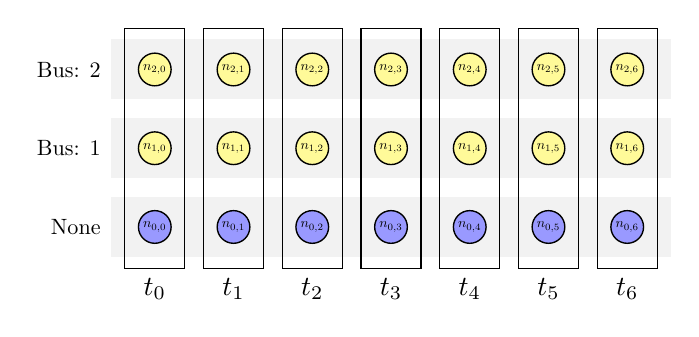
\begin{tikzpicture}
	\node[rectangle, fill=gray!10, minimum width=2.8in, minimum height=.3in,label=left:\scalebox{0.8}{Bus: 2}](bus2Box) at (3,1){};
	\node[rectangle, fill=gray!10, minimum width=2.8in, minimum height=.3in,label=left:\scalebox{0.8}{Bus: 1}](bus1Box) at (3,0){};
	\node[rectangle, fill=gray!10, minimum width=2.8in, minimum height=.3in,label=left:\scalebox{0.8}{None}](bus1Box) at (3,-1){};

	\node[circle, fill=yellow!40, line width=0.5pt, draw=black, minimum size=0.15in, inner sep=1pt](one) at (0,0){\scalebox{0.5}{$n_{1,0}$}};
	\node[circle, fill=yellow!40, line width=0.5pt, draw=black, minimum size=0.15in, inner sep=1pt](two) at (1,0){\scalebox{0.5}{$n_{1,1}$}}; 
	\node[circle, fill=yellow!40, line width=0.5pt, draw=black, minimum size=0.15in, inner sep=1pt](three) at (2,0){\scalebox{0.5}{$n_{1,2}$}};
	\node[circle, fill=yellow!40, line width=0.5pt, draw=black, minimum size=0.15in, inner sep=1pt](four) at (3,0){\scalebox{0.5}{$n_{1,3}$}};
	\node[circle, fill=yellow!40, line width=0.5pt, draw=black, minimum size=0.15in, inner sep=1pt](five) at (4,0){\scalebox{0.5}{$n_{1,4}$}};
	\node[circle, fill=yellow!40, line width=0.5pt, draw=black, minimum size=0.15in, inner sep=1pt](six) at (5,0){\scalebox{0.5}{$n_{1,5}$}};
	\node[circle, fill=yellow!40, line width=0.5pt, draw=black, minimum size=0.15in, inner sep=1pt](seven) at (6,0){\scalebox{0.5}{$n_{1,6}$}};

	\node[circle, fill=yellow!40, line width=0.5pt, draw=black, minimum size=0.15in, inner sep=1pt](eight) at (0,1){\scalebox{0.5}{$n_{2,0}$}};
	\node[circle, fill=yellow!40, line width=0.5pt, draw=black, minimum size=0.15in, inner sep=1pt](nine) at (1,1){\scalebox{0.5}{$n_{2,1}$}}; 
	\node[circle, fill=yellow!40, line width=0.5pt, draw=black, minimum size=0.15in, inner sep=1pt](ten) at (2,1){\scalebox{0.5}{$n_{2,2}$}};
	\node[circle, fill=yellow!40, line width=0.5pt, draw=black, minimum size=0.15in, inner sep=1pt](eleven) at (3,1){\scalebox{0.5}{$n_{2,3}$}};
	\node[circle, fill=yellow!40, line width=0.5pt, draw=black, minimum size=0.15in, inner sep=1pt](twelve) at (4,1){\scalebox{0.5}{$n_{2,4}$}};
	\node[circle, fill=yellow!40, line width=0.5pt, draw=black, minimum size=0.15in, inner sep=1pt](thirteen) at (5,1){\scalebox{0.5}{$n_{2,5}$}};
	\node[circle, fill=yellow!40, line width=0.5pt, draw=black, minimum size=0.15in, inner sep=1pt](fourteen) at (6,1){\scalebox{0.5}{$n_{2,6}$}};

	\node[circle, fill=blue!40, line width=0.5pt, draw=black, minimum size=0.15in, inner sep=1pt](eight) at (0,-1){\scalebox{0.5}{$n_{0,0}$}};
	\node[circle, fill=blue!40, line width=0.5pt, draw=black, minimum size=0.15in, inner sep=1pt](nine) at (1,-1){\scalebox{0.5}{$n_{0,1}$}}; 
	\node[circle, fill=blue!40, line width=0.5pt, draw=black, minimum size=0.15in, inner sep=1pt](ten) at (2,-1){\scalebox{0.5}{$n_{0,2}$}};
	\node[circle, fill=blue!40, line width=0.5pt, draw=black, minimum size=0.15in, inner sep=1pt](eleven) at (3,-1){\scalebox{0.5}{$n_{0,3}$}};
	\node[circle, fill=blue!40, line width=0.5pt, draw=black, minimum size=0.15in, inner sep=1pt](twelve) at (4,-1){\scalebox{0.5}{$n_{0,4}$}};
	\node[circle, fill=blue!40, line width=0.5pt, draw=black, minimum size=0.15in, inner sep=1pt](thirteen) at (5,-1){\scalebox{0.5}{$n_{0,5}$}};
	\node[circle, fill=blue!40, line width=0.5pt, draw=black, minimum size=0.15in, inner sep=1pt](fourteen) at (6,-1){\scalebox{0.5}{$n_{0,6}$}};

	\node[rectangle, draw, minimum width=0.3in, minimum height=1.2in,label=below:$t_0$](time0Box) at (0,0){};
	\node[rectangle, draw, minimum width=0.3in, minimum height=1.2in,label=below:$t_1$](time1Box) at (1,0){};
	\node[rectangle, draw, minimum width=0.3in, minimum height=1.2in,label=below:$t_2$](time2Box) at (2,0){};
	\node[rectangle, draw, minimum width=0.3in, minimum height=1.2in,label=below:$t_3$](time3Box) at (3,0){};
	\node[rectangle, draw, minimum width=0.3in, minimum height=1.2in,label=below:$t_4$](time4Box) at (4,0){};
	\node[rectangle, draw, minimum width=0.3in, minimum height=1.2in,label=below:$t_5$](time5Box) at (5,0){};
	\node[rectangle, draw, minimum width=0.3in, minimum height=1.2in,label=below:$t_6$](time6Box) at (6,0){}; 
\end{tikzpicture}
	\caption{Grid of nodes showing discrete timesteps advancing from left to right and charger states ascending vertically.}
	\label{fig:graphGridStructure} 
\end{figure}
\begin{figure}
\centering
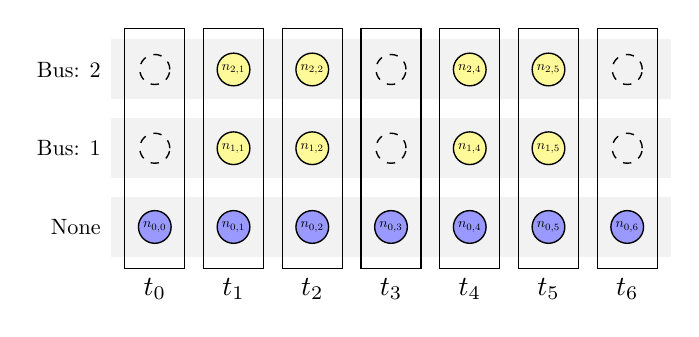
\begin{tikzpicture} 
	\node[rectangle, fill=gray!10, minimum width=2.8in, minimum height=.3in,label=left:\scalebox{0.8}{Bus: 2}](bus2Box) at (3,1){};
	\node[rectangle, fill=gray!10, minimum width=2.8in, minimum height=.3in,label=left:\scalebox{0.8}{Bus: 1}](bus1Box) at (3,0){};
	\node[rectangle, fill=gray!10, minimum width=2.8in, minimum height=.3in,label=left:\scalebox{0.8}{None}](bus1Box) at (3,-1){};

	\node[circle, draw, dashed,   line width=0.5pt, draw=black, minimum size=0.15in, inner sep=1pt](one)   at (0,0){};
	\node[circle, fill=yellow!40, line width=0.5pt, draw=black, minimum size=0.15in, inner sep=1pt](two)   at (1,0){\scalebox{0.5}{$n_{1,1}$}}; 
	\node[circle, fill=yellow!40, line width=0.5pt, draw=black, minimum size=0.15in, inner sep=1pt](three) at (2,0){\scalebox{0.5}{$n_{1,2}$}};
	\node[circle, draw, dashed,   line width=0.5pt, draw=black, minimum size=0.15in, inner sep=1pt](four)  at (3,0){};
	\node[circle, fill=yellow!40, line width=0.5pt, draw=black, minimum size=0.15in, inner sep=1pt](five)  at (4,0){\scalebox{0.5}{$n_{1,4}$}};
	\node[circle, fill=yellow!40, line width=0.5pt, draw=black, minimum size=0.15in, inner sep=1pt](six)   at (5,0){\scalebox{0.5}{$n_{1,5}$}};
	\node[circle, draw, dashed,   line width=0.5pt, draw=black, minimum size=0.15in, inner sep=1pt](seven) at (6,0){};

	\node[circle, draw, dashed,   line width=0.5pt, draw=black, minimum size=0.15in, inner sep=1pt](eight)    at (0,1){};
	\node[circle, fill=yellow!40, line width=0.5pt, draw=black, minimum size=0.15in, inner sep=1pt](nine)     at (1,1){\scalebox{0.5}{$n_{2,1}$}}; 
	\node[circle, fill=yellow!40, line width=0.5pt, draw=black, minimum size=0.15in, inner sep=1pt](ten)      at (2,1){\scalebox{0.5}{$n_{2,2}$}};
	\node[circle, draw, dashed,   line width=0.5pt, draw=black, minimum size=0.15in, inner sep=1pt](eleven)   at (3,1){};
	\node[circle, fill=yellow!40, line width=0.5pt, draw=black, minimum size=0.15in, inner sep=1pt](twelve)   at (4,1){\scalebox{0.5}{$n_{2,4}$}};
	\node[circle, fill=yellow!40, line width=0.5pt, draw=black, minimum size=0.15in, inner sep=1pt](thirteen) at (5,1){\scalebox{0.5}{$n_{2,5}$}};
	\node[circle, draw, dashed,   line width=0.5pt, draw=black, minimum size=0.15in, inner sep=1pt](fourteen) at (6,1){};

	\node[circle, fill=blue!40,   line width=0.5pt, draw=black, minimum size=0.15in, inner sep=1pt](eight)    at (0,-1){\scalebox{0.5}{$n_{0,0}$}};
	\node[circle, fill=blue!40,   line width=0.5pt, draw=black, minimum size=0.15in, inner sep=1pt](nine)     at (1,-1){\scalebox{0.5}{$n_{0,1}$}}; 
	\node[circle, fill=blue!40,   line width=0.5pt, draw=black, minimum size=0.15in, inner sep=1pt](ten)      at (2,-1){\scalebox{0.5}{$n_{0,2}$}};
	\node[circle, fill=blue!40,   line width=0.5pt, draw=black, minimum size=0.15in, inner sep=1pt](eleven)   at (3,-1){\scalebox{0.5}{$n_{0,3}$}};
	\node[circle, fill=blue!40,   line width=0.5pt, draw=black, minimum size=0.15in, inner sep=1pt](twelve)   at (4,-1){\scalebox{0.5}{$n_{0,4}$}};
	\node[circle, fill=blue!40,   line width=0.5pt, draw=black, minimum size=0.15in, inner sep=1pt](thirteen) at (5,-1){\scalebox{0.5}{$n_{0,5}$}};
	\node[circle, fill=blue!40,   line width=0.5pt, draw=black, minimum size=0.15in, inner sep=1pt](fourteen) at (6,-1){\scalebox{0.5}{$n_{0,6}$}};

	\node[rectangle, draw, minimum width=0.3in, minimum height=1.2in,label=below:$t_0$](time0Box) at (0,0){};
	\node[rectangle, draw, minimum width=0.3in, minimum height=1.2in,label=below:$t_1$](time1Box) at (1,0){};
	\node[rectangle, draw, minimum width=0.3in, minimum height=1.2in,label=below:$t_2$](time2Box) at (2,0){};
	\node[rectangle, draw, minimum width=0.3in, minimum height=1.2in,label=below:$t_3$](time3Box) at (3,0){};
	\node[rectangle, draw, minimum width=0.3in, minimum height=1.2in,label=below:$t_4$](time4Box) at (4,0){};
	\node[rectangle, draw, minimum width=0.3in, minimum height=1.2in,label=below:$t_5$](time5Box) at (5,0){};
	\node[rectangle, draw, minimum width=0.3in, minimum height=1.2in,label=below:$t_6$](time6Box) at (6,0){}; 
\end{tikzpicture}
	\caption{Grid of nodes displaying times when buses are available for charging.}
	\label{fig:busAvailComparison}
\end{figure}

\par The state of a charger at any time is represented by existing in a particular node. Changes in charger state over time are represented by the transitions from a node to multiple possible next nodes. These transitions are called edges (see Fig.~\ref{fig:edgeNodeRel}) and represent four possible decisions: connect to a bus, charge a bus, remain idle, or disconnect from a bus. Edges are associated with actions and that action is determined by the nodes on either end. Consider the edge from $n_{0,0}$ to $n_{0,1}$ in Fig.~\ref{fig:edgeTypes}. This edge represents a no-charge decision because the nodes on both ends represent the disconnected charge state at times $t_0$ and $t_1$. Chargers cannot charge while disconnected, so the edge decision is no-charge.  Similarly, the edge between $n_{1,1}$ and $n_{1,2}$ indicates a decision to-charge as both $n_{1,1}$ and $n_{1,2}$ represent states where a charger is connected at times $t_1$ and $t_2$. Both to-charge and no-charge decisions are represented by \textit{horizontal} transitions in the graph and only reflect the passing of time as no changes to the physical hardware are made.
\par Conversely, diagonal transitions imply physical hardware changes because they represent decisions where chargers connect to or disconnect from a bus. One such example from Fig.~\ref{fig:edgeTypes} includes the edge from $n_{0,0}$ to $n_{1,1}$. The state represented by $n_{0,0}$ is disconnected This edge represents an interval where a charger is disconnected at $t_0$ and connected at $t_1$, implying a `to-connect' decision. The same logic applies in reverse for the edge between $n_{1,2}$ and $n_{0,3}$. Hence, the bus charge problem can be described in terms of nodes and edges (i.e. a graph) where nodes represent bus availability for charging and edges encode all possible charge decisions. 
\par A charge schedule can be thought of as a list of charge decisions that govern charge behavior. Because decisions are represented by edges in the graph, a schedule is also represented by a sequence of connected edges that form a path through the graph. If an edge is selected, or active, it is considered part of the path.  Active and inactive edges are represented edge weights equal to $1$ and $0$, respectively.
\par A graph with binary edge weights can only represent a plan for one charger. This representation can be expanded to represent an arbitrary number of chargers by using integer valued weights, where each weight gives the number of chargers in the transition.
\begin{figure}
	\centering
	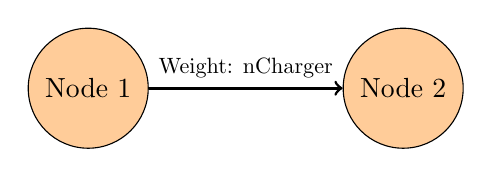
\begin{tikzpicture}
		\node[circle, draw, fill=orange!40, minimum size=0.6in](node1) at (0,0){Node 1};
		\node[circle, draw, fill=orange!40, minimum size=0.6in](node2) at (4,0){Node 2};
		\draw [->, line width=1pt] (node1.east) -- node[above]{\scalebox{0.8}{Weight: nCharger}}(node2.west); 
	\end{tikzpicture}
	\caption{Node to node connection.}
	\label{fig:edgeNodeRel}
\end{figure} 
\begin{figure}
	\centering
	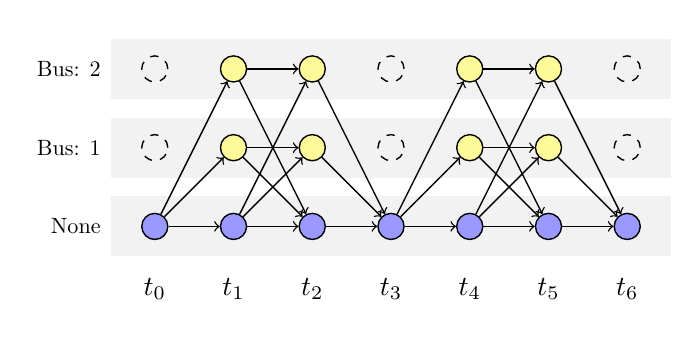
\begin{tikzpicture} 
		\node[rectangle, fill=gray!10, minimum width=2.8in, minimum height=.3in,label=left:\scalebox{0.8}{Bus: 2}](bus2Box) at (3,1){};
		\node[rectangle, fill=gray!10, minimum width=2.8in, minimum height=.3in,label=left:\scalebox{0.8}{Bus: 1}](bus1Box) at (3,0){};
		\node[rectangle, fill=gray!10, minimum width=2.8in, minimum height=.3in,label=left:\scalebox{0.8}{None}](bus1Box) at (3,-1){};

		\node[circle, draw, dashed, line width=0.5pt, draw=black, minimum size=0.1in](one) at (0,0){};
		\node[circle, fill=yellow!40, line width=0.5pt, draw=black, minimum size=0.1in](two) at (1,0){}; 
		\node[circle, fill=yellow!40, line width=0.5pt, draw=black, minimum size=0.1in](three) at (2,0){};
		\node[circle, draw, dashed, line width=0.5pt, draw=black, minimum size=0.1in](four) at (3,0){};
		\node[circle, fill=yellow!40, line width=0.5pt, draw=black, minimum size=0.1in](five) at (4,0){};
		\node[circle, fill=yellow!40, line width=0.5pt, draw=black, minimum size=0.1in](six) at (5,0){};
		\node[circle, draw, dashed,  line width=0.5pt, draw=black, minimum size=0.1in](seven) at (6,0){};

		\node[circle, draw, dashed, line width=0.5pt, draw=black, minimum size=0.1in](eight) at (0,1){};
		\node[circle, fill=yellow!40, line width=0.5pt, draw=black, minimum size=0.1in](nine) at (1,1){}; 
		\node[circle, fill=yellow!40, line width=0.5pt, draw=black, minimum size=0.1in](ten) at (2,1){};
		\node[circle, draw, dashed, line width=0.5pt, draw=black, minimum size=0.1in](eleven) at (3,1){};
		\node[circle, fill=yellow!40, line width=0.5pt, draw=black, minimum size=0.1in](twelve) at (4,1){};
		\node[circle, fill=yellow!40, line width=0.5pt, draw=black, minimum size=0.1in](thirteen) at (5,1){};
		\node[circle, draw, dashed, line width=0.5pt, draw=black, minimum size=0.1in](fourteen) at (6,1){};

		\node[circle, fill=blue!40, line width=0.5pt, draw=black, minimum size=0.1in](bOne) at (0,-1){};
		\node[circle, fill=blue!40, line width=0.5pt, draw=black, minimum size=0.1in](bTwo) at (1,-1){}; 
		\node[circle, fill=blue!40, line width=0.5pt, draw=black, minimum size=0.1in](bThree) at (2,-1){};
		\node[circle, fill=blue!40, line width=0.5pt, draw=black, minimum size=0.1in](bFour) at (3,-1){};
		\node[circle, fill=blue!40, line width=0.5pt, draw=black, minimum size=0.1in](bFive) at (4,-1){};
		\node[circle, fill=blue!40, line width=0.5pt, draw=black, minimum size=0.1in](bSix) at (5,-1){};
		\node[circle, fill=blue!40, line width=0.5pt, draw=black, minimum size=0.1in](bSeven) at (6,-1){};

		\node[rectangle, minimum width=0.3in, minimum height=1.2in,label=below:$t_0$](time0Box) at (0,0){};
		\node[rectangle, minimum width=0.3in, minimum height=1.2in,label=below:$t_1$](time1Box) at (1,0){};
		\node[rectangle, minimum width=0.3in, minimum height=1.2in,label=below:$t_2$](time2Box) at (2,0){};
		\node[rectangle, minimum width=0.3in, minimum height=1.2in,label=below:$t_3$](time3Box) at (3,0){};
		\node[rectangle, minimum width=0.3in, minimum height=1.2in,label=below:$t_4$](time4Box) at (4,0){};
		\node[rectangle, minimum width=0.3in, minimum height=1.2in,label=below:$t_5$](time5Box) at (5,0){};
		\node[rectangle, minimum width=0.3in, minimum height=1.2in,label=below:$t_6$](time6Box) at (6,0){}; 
		
		% draw rest edges
		\draw[->, line width=0.5pt] (bOne) -- (bTwo);
		\draw[->, line width=0.5pt] (bTwo) -- (bThree);
		\draw[->, line width=0.5pt] (bThree) -- (bFour);
		\draw[->, line width=0.5pt] (bFour) -- (bFive);
		\draw[->, line width=0.5pt] (bFive) -- (bSix);
		\draw[->, line width=0.5pt] (bSix) -- (bSeven);
		
		% draw connect edges
		\draw[->, line width=0.5pt] (bOne) -- (two); 
		\draw[->, line width=0.5pt] (bTwo) -- (three);
		\draw[->, line width=0.5pt] (bFour) -- (five);
		\draw[->, line width=0.5pt] (bFive) -- (six);

		\draw[->, line width=0.5pt] (bOne) -- (nine);
		\draw[->, line width=0.5pt] (bTwo) -- (ten);
		\draw[->, line width=0.5pt] (bFour) -- (twelve);
		\draw[->, line width=0.5pt] (bFive) -- (thirteen);

		% draw disconnect edges
		\draw[->, line width=0.5pt] (two) -- (bThree); 
		\draw[->, line width=0.5pt] (three) -- (bFour);
		\draw[->, line width=0.5pt] (five) -- (bSix);
		\draw[->, line width=0.5pt] (six) -- (bSeven);

		\draw[->, line width=0.5pt] (nine) -- (bThree);
		\draw[->, line width=0.5pt] (ten) -- (bFour);
		\draw[->, line width=0.5pt] (twelve) -- (bSix);
		\draw[->, line width=0.5pt] (thirteen) -- (bSeven);

		% draw charge edges
		\draw[->, line width=0.5pt] (two) -- (three);
		\draw[->, line width=0.5pt] (five) -- (six);
		\draw[->, line width=0.5pt] (nine) -- (ten);
		\draw[->, line width=0.5pt] (twelve) -- (thirteen);

	\end{tikzpicture}
	\caption{Graph-based model of the complete decision-space.}
	\label{fig:completeGraph}
\end{figure}
\begin{figure}
	\centering
	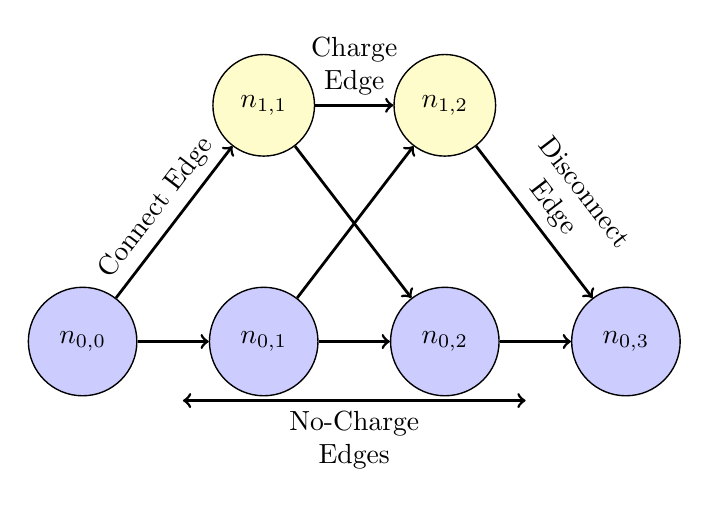
\begin{tikzpicture}
		\node[circle, fill=blue!20,line width=0.5pt, draw=black, text width=0.5in, inner sep=1pt,   align=center](one)   at (0,0)  {$n_{0,0}$};
		\node[circle, fill=blue!20,line width=0.5pt, draw=black, text width=0.5in, inner sep=1pt,   align=center](two)   at (2.3,0){$n_{0,1}$};
		\node[circle, fill=blue!20,line width=0.5pt, draw=black, text width=0.5in, inner sep=1pt,   align=center](three) at (4.6,0){$n_{0,2}$};
		\node[circle, fill=blue!20,line width=0.5pt, draw=black, text width=0.5in, inner sep=1pt,   align=center](four)  at (6.9,0){$n_{0,3}$};
		\node[circle, fill=yellow!20,line width=0.5pt, draw=black, text width=0.5in, inner sep=0in, align=center](five)  at (2.3,3){$n_{1,1}$};
		\node[circle, fill=yellow!20,line width=0.5pt, draw=black, text width=0.5in, inner sep=0in, align=center](six)   at (4.6,3){$n_{1,2}$};
		\node(placeholder1) at (1.15,-0.75){};
		\node(placeholder2) at (5.75,-0.75){};
		\draw [->, line width=1pt] (one) -- node[sloped, anchor=center, above, text width=2.5cm, midway, align=center]{Connect Edge}(five);
		\draw [->, line width=1pt] (one) -- (two);
		\draw [->, line width=1pt] (five) -- node[sloped, anchor=center, above, text width=1.5cm, midway, align=center]{Charge Edge}(six);
		\draw [->, line width=1pt] (five) -- (three);
		\draw [->, line width=1pt] (two) -- (six);
		\draw [->, line width=1pt] (six) -- node[sloped, anchor=center, above, text width=1.5cm, midway, align=center]{Disconnect Edge}(four);
		\draw [->, line width=1pt] (two) -- (three);
		\draw [->, line width=1pt] (three) -- (four); 
		\draw [<->, line width=1pt] (placeholder1) -- node[below, text width=2cm, midway, align=center]{No-Charge Edges}(placeholder2);
	\end{tikzpicture}
	\caption{Illustrates different types of edges: connect, disconnect, and charge edges.}
	\label{fig:edgeTypes}
\end{figure} 
\par Consider a three-charger scenario using the graph in Fig.~\ref{fig:completeGraph}. A solution where one charger is connected to Bus 1 from $t_1$ to $t_2$ and to Bus 2 from $t_4$ to $t_5$ would be expressed by assigning unit weights to the appropriate connect, charge, and disconnect edges.  The second charger remains idle as illustrated by the active edges along the bottom row of charger states (see Fig.~\ref{fig:graphWithSolution}).  
\par In summary, the graph encodes bus availability with nodes, decisions with edges, and schedules with edge weights. Solving the bus charge problem becomes a matter of finding the optimal set of edge weights, where optimal is meant to denote the most cost effective charge plan.

\begin{figure}
	\centering
	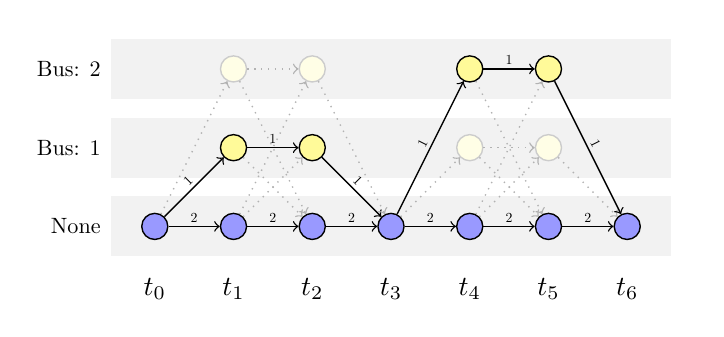
\begin{tikzpicture} 
		\node[rectangle, fill=gray!10, minimum width=2.8in, minimum height=.3in,label=left:\scalebox{0.8}{Bus: 2}](bus2Box) at (3,1){};
		\node[rectangle, fill=gray!10, minimum width=2.8in, minimum height=.3in,label=left:\scalebox{0.8}{Bus: 1}](bus1Box) at (3,0){};
		\node[rectangle, fill=gray!10, minimum width=2.8in, minimum height=.3in,label=left:\scalebox{0.8}{None}](bus1Box) at (3,-1){};

		\node[circle, fill=yellow!40, line width=0.5pt, draw=black, minimum size=0.1in](two) at (1,0){}; 
		\node[circle, fill=yellow!40, line width=0.5pt, draw=black, minimum size=0.1in](three) at (2,0){};
		\node[circle, fill=yellow!10, line width=0.5pt, draw=black!20, minimum size=0.1in](five) at (4,0){};
		\node[circle, fill=yellow!10, line width=0.5pt, draw=black!20, minimum size=0.1in](six) at (5,0){};

		\node[circle, fill=yellow!10, line width=0.5pt, draw=black!20, minimum size=0.1in](nine) at (1,1){}; 
		\node[circle, fill=yellow!10, line width=0.5pt, draw=black!20, minimum size=0.1in](ten) at (2,1){};
		\node[circle, fill=yellow!40, line width=0.5pt, draw=black, minimum size=0.1in](twelve) at (4,1){};
		\node[circle, fill=yellow!40, line width=0.5pt, draw=black, minimum size=0.1in](thirteen) at (5,1){};

		\node[circle, fill=blue!40, line width=0.5pt, draw=black, minimum size=0.1in](bOne) at (0,-1){};
		\node[circle, fill=blue!40, line width=0.5pt, draw=black, minimum size=0.1in](bTwo) at (1,-1){}; 
		\node[circle, fill=blue!40, line width=0.5pt, draw=black, minimum size=0.1in](bThree) at (2,-1){};
		\node[circle, fill=blue!40, line width=0.5pt, draw=black, minimum size=0.1in](bFour) at (3,-1){};
		\node[circle, fill=blue!40, line width=0.5pt, draw=black, minimum size=0.1in](bFive) at (4,-1){};
		\node[circle, fill=blue!40, line width=0.5pt, draw=black, minimum size=0.1in](bSix) at (5,-1){};
		\node[circle, fill=blue!40, line width=0.5pt, draw=black, minimum size=0.1in](bSeven) at (6,-1){};

		\node[rectangle, minimum width=0.3in, minimum height=1.2in,label=below:$t_0$](time0Box) at (0,0){};
		\node[rectangle, minimum width=0.3in, minimum height=1.2in,label=below:$t_1$](time1Box) at (1,0){};
		\node[rectangle, minimum width=0.3in, minimum height=1.2in,label=below:$t_2$](time2Box) at (2,0){};
		\node[rectangle, minimum width=0.3in, minimum height=1.2in,label=below:$t_3$](time3Box) at (3,0){};
		\node[rectangle, minimum width=0.3in, minimum height=1.2in,label=below:$t_4$](time4Box) at (4,0){};
		\node[rectangle, minimum width=0.3in, minimum height=1.2in,label=below:$t_5$](time5Box) at (5,0){};
		\node[rectangle, minimum width=0.3in, minimum height=1.2in,label=below:$t_6$](time6Box) at (6,0){}; 
		
		% draw rest edges
		\draw[->, line width=0.5pt] (bOne) -- node [text width=2.5cm, midway, above=-2.1pt, align=center]{\scalebox{0.5}{2}}(bTwo);
		\draw[->, line width=0.5pt] (bTwo) -- node [text width=2.5cm, midway, above=-2.1pt, align=center]{\scalebox{0.5}{2}}(bThree);
		\draw[->, line width=0.5pt] (bThree) -- node [text width=2.5cm, midway, above=-2.1pt, align=center]{\scalebox{0.5}{2}}(bFour);
		\draw[->, line width=0.5pt] (bFour) -- node [text width=2.5cm, midway, above=-2.1pt, align=center]{\scalebox{0.5}{2}}(bFive);
		\draw[->, line width=0.5pt] (bFive) -- node [text width=2.5cm, midway, above=-2.1pt, align=center]{\scalebox{0.5}{2}}(bSix);
		\draw[->, line width=0.5pt] (bSix) -- node [text width=2.5cm, midway, above=-2.1pt, align=center]{\scalebox{0.5}{2}}(bSeven);
		
		% draw connect edges
		\draw[->, line width=0.5pt] (bOne) -- node [sloped, text width=2.5cm, midway, above=-2.1pt, align=center]{\scalebox{0.5}{1}}(two); 
		\draw[->, dotted, color=black!30, line width=0.5pt] (bTwo) -- (three);
		\draw[->, dotted, color=black!30, line width=0.5pt] (bFour) -- (five);
		\draw[->, dotted, color=black!30, line width=0.5pt] (bFive) -- (six);

		\draw[->, dotted, color=black!30, line width=0.5pt] (bOne) -- (nine);
		\draw[->, dotted, color=black!30, line width=0.5pt] (bTwo) -- (ten);
		\draw[->, line width=0.5pt] (bFour) -- node [sloped, text width=2.5cm, midway, above=-2.1pt, align=center]{\scalebox{0.5}{1}}(twelve);
		\draw[->, dotted, color=black!30, line width=0.5pt] (bFive) -- (thirteen);

		% draw disconnect edges
		\draw[->, dotted, color=black!30, line width=0.5pt] (two) -- (bThree); 
		\draw[->, line width=0.5pt] (three) -- node [sloped, text width=2.5cm, midway, above=-2.1pt, align=center]{\scalebox{0.5}{1}}(bFour);
		\draw[->, dotted, color=black!30, line width=0.5pt] (five) -- (bSix);
		\draw[->, dotted, color=black!30, line width=0.5pt] (six) -- (bSeven);

		\draw[->, dotted, color=black!30, line width=0.5pt] (nine) -- (bThree);
		\draw[->, dotted, color=black!30, line width=0.5pt] (ten) -- (bFour);
		\draw[->, dotted, color=black!30, line width=0.5pt] (twelve) -- (bSix);
		\draw[->, line width=0.5pt] (thirteen) -- node [sloped, text width=2.5cm, midway, above=-2.1pt, align=center]{\scalebox{0.5}{1}}(bSeven);

		% draw charge edges
		\draw[->, line width=0.5pt] (two) -- node [text width=2.5cm, midway, above=-2.1pt, align=center]{\scalebox{0.5}{1}}(three);
		\draw[->, dotted, color=black!30, line width=0.5pt] (five) -- (six);
		\draw[->, dotted, color=black!30, line width=0.5pt] (nine) -- (ten);
		\draw[->, line width=0.5pt] (twelve) -- node [text width=2.5cm, midway, above=-2.1pt, align=center]{\scalebox{0.5}{1}}(thirteen); 
	\end{tikzpicture}
	\caption{A solution to a 2-bus 3-charger scenario.}
	\label{fig:graphWithSolution}
\end{figure}

\subsection{Graph Constraints}
\par Finding the optimal charge schedule can be expressed as an optimization problem, where the graph is used to derive equality and inequality constraints for a mixed integer linear program (MILP)
\begin{equation}
	\begin{aligned}
		& \underset{\mathbf{y}}{\text{min}}\ \mathbf{r}^T\mathbf{y} \ \text{subject to} \\
		& F\mathbf{y} = \mathbf{f}, \ Q\mathbf{y} \le \mathbf{q},
	\end{aligned}
\end{equation}
where the equality and inequality constraints are encoded in $F$, $\mathbf{f}$, $Q$ and $\mathbf{q}$. The variable $\mathbf{y}$ is a vector containing the elements of the solution and has the form 
\begin{equation}\label{eqn:y}
		\mathbf{y}^T = \begin{bmatrix}
		\mathbf{x}^T  \
		\mathbf{d}^T  \
		\mathbf{g}^T  \
		\mathbf{e}^T  \
		\mathbf{p}^T  \
		\hat{p}  \
		\hat{p}_\text{off-peak}  \
		\hat{p}_\text{on-peak}  \
	\end{bmatrix},
\end{equation}
where each element of $\mathbf{y}$ is defined later in this paper.
\par  This subsection formulates two sets of constraints.  The first represents the graph structure, enforces conservation of chargers, and defines the number of chargers through a set of net-flow constraints. The second prevents the charger from thrashing between connected/disconnected states and enforces one-bus/one-charger connectivity by enforcing what we call ``group flow'' constraints.
\subsubsection{\label{sec:net-flow} Net-Flow Constraints}
Network flow constraints are expressed in matrix-vector form as
\begin{align}\label{eqn:flow}
	A\mathbf{x}=\mathbf{c}_f,	
\end{align}
where $A$ is the graph incidence matrix, $\mathbf{x}$ is the $n_E \times 1$ vector of edge weights and corresponds to $\mathbf{x}$ in equation \ref{eqn:y}, and $\mathbf{c}_f$ is $n_N \times 1$ and equals the difference between incoming and outgoing edge weights, or \textit{net-flow}.  The parameter $n_E$ is the number of edges and $n_N$ is the number of nodes.
\par  An incidence matrix organizes relationships between nodes and edges by describing which edges leave and enter which nodes. The matrix $A$ is an $n_N \times n_E$ matrix and expresses incoming connections between the $i^{\text{th}}$ node and $j^{\text{th}}$ edge by $A_{i,j} = 1$. Similarly, outgoing connections are given by $A_{i,j} = -1$, and no connection with $A_{i,j} = 0$. For example, the graph in Fig. \ref{fig:genericGraph} is represented as:
\begin{figure}
	\centering
	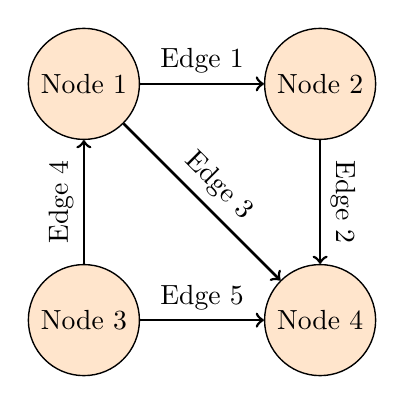
\begin{tikzpicture}
		\node[circle, line width=0.5pt, draw=black, fill=orange!20, minimum size=0.5in](topLeft) at (0,3){Node 1};
		\node[circle, line width=0.5pt, draw=black, fill=orange!20, minimum size=0.5in](topRight) at (3,3){Node 2};
		\node[circle, line width=0.5pt, draw=black, fill=orange!20, minimum size=0.5in](btmLeft) at (0,0){Node 3};
		\node[circle, line width=0.5pt, draw=black, fill=orange!20, minimum size=0.5in](btmRight) at (3,0){Node 4};
		\draw [->, line width=1pt] (topLeft.east) -- node [text width=2.5cm, midway, above, align=center]{Edge 1}(topRight.west);
		\draw [->, line width=1pt] (btmLeft.north) -- node [sloped, anchor=center, above, text width=2.5cm, midway, align=center]{Edge 4}(topLeft.south);
		\draw [->, line width=1pt] (topLeft.south east) -- node [sloped, anchor=center, above, text width=2.5cm, midway, align=center]{Edge 3}(btmRight.north west);
		\draw [->, line width=1pt] (topRight.south) -- node[sloped, anchor=center, above, text width=2.5cm, midway, align=center]{Edge 2}(btmRight.north);
		\draw [->, line width=1pt] (btmLeft.east) -- node[text width=2.5cm, midway, above, align=center]{Edge 5}(btmRight.west);
	\end{tikzpicture}
	\caption{A generic directed graph consisting of nodes and edges.}
	\label{fig:genericGraph}
\end{figure}
\begin{align}
	\begin{bmatrix}
		-1 & 0 & -1 & 1 & 0 \\
		1 & -1 & 0 & 0 & 0 \\
		0 & 0 & 0 & -1 & -1 \\
		0 & 1 & 1 & 0 & 1 \\
	\end{bmatrix}
\end{align}
\par  The difference between the number of chargers entering and leaving, or the \textit{net-flow}, can be expressed in terms of $A$ as seen in equation (\ref{eqn:flow}).  Because the number of chargers does not change, the number of chargers entering and leaving a node must be equal. This is expressed in linear form as $a_i^{T}x = 0$, where $a_i$ is the $i^{\text{th}}$ row of $A$. The only exceptions occur at \textit{source} and \textit{sink} nodes.
\par A source node represents the beginning state for all chargers.  Because edges originate here, there are no incoming edges and the net-flow will be minus the number of chargers. This is described in linear form as $a_i^Tx = -n_C$, where $n_C$ is the number of chargers.
\par Sink nodes represent the final state, where all edges terminate (see Fig.~\ref{fig:sourceSink}). Because sinks have no outgoing edges, they maintain a positive net-flow equal to the number of chargers and is expressed by $a_i^T = n_C$. 
\par Therefore, the \textit{flow constraints} require the elements of $\mathbf{c}_f$ be equal to zero for all non-source and non-sink nodes as seen in equation (\ref{eqn:cFlow}).  
\begin{figure}
	\centering
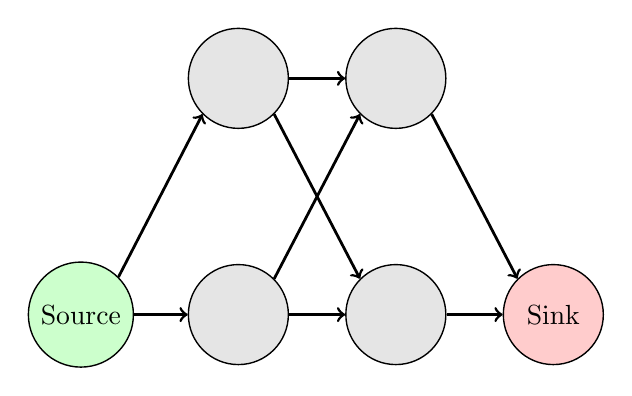
\begin{tikzpicture}
	\node[circle, fill=green!20, line width=0.5pt, draw=black, minimum size=0.5in](one) at (0,0){Source};
	\node[circle, fill=gray!20,line width=0.5pt, draw=black, minimum size=0.5in](two) at (2,0){};
	\node[circle, fill=gray!20,line width=0.5pt, draw=black, minimum size=0.5in](three) at (4,0){};
	\node[circle, fill=red!20,line width=0.5pt, draw=black, minimum size=0.5in](four) at (6,0){Sink};
	\node[circle, fill=gray!20, line width=0.5pt, draw=black, minimum size=0.5in](five) at (2,3){};
	\node[circle, fill=gray!20, line width=0.5pt, draw=black, minimum size=0.5in](six) at (4,3){};
	\draw [->, line width=1pt] (one.north east) -- (five.south west);
	\draw [->, line width=1pt] (one.east) -- (two.west);
	\draw [->, line width=1pt] (five.east) -- (six.west);
	\draw [->, line width=1pt] (five.south east) -- (three.north west);
	\draw [->, line width=1pt] (two.north east) -- (six.south west);
	\draw [->, line width=1pt] (six.south east) -- (four.north west);
	\draw [->, line width=1pt] (two.east) -- (three.west);
	\draw [->, line width=1pt] (three.east) -- (four.west); 
\end{tikzpicture}
	\caption{Network flow illustrating sources and sinks.}
	\label{fig:sourceSink} 
\end{figure} 
\begin{align}\label{eqn:cFlow}
	Ax = \begin{bmatrix} 0  \ \hdots \ -n_C \ \hdots \ 0 \ n_C \ \hdots \ 0\end{bmatrix}^T.
\end{align}
Equation \ref{eqn:cFlow} can be formulated in terms of $\mathbf{y}$ by appropriately zero-padding $A$ such that
\begin{equation}\label{eqn:cFlow2}
	\begin{aligned}
		c_f &= \begin{bmatrix}A & 0 \end{bmatrix}\mathbf{y}\\
		    &= \tilde{A} \mathbf{y} 
	\end{aligned}
\end{equation}
\subsubsection{Group-flow Constraints}
\par Another flow type, known as group flow, can be used to regulate the number of chargers entering a set of nodes. This is desired for two reasons.  First, it prevents chargers from connecting multiple times during an interval when a bus is available for charging, and it limits the number of chargers connecting to a bus to be one at most.
\par Define a charge group as the set of all nodes for a given bus corresponding to one station visit as shown in Fig.~\ref{fig:groups}. The \textit{group flow} is the number of chargers that enter a group and is represented as the sum of all incoming edge weights (see Fig. \ref{fig:groupedEdges}). 
\par Denote the $n_G \times n_E$ group incidence matrix as $B$, where $n_G$ is the number of groups and $B_{i,j}$ is $1$ if the $j^{\text{th}}$ edge enters the $i^{\text{th}}$ group and $0$ otherwise. For example, the group incidence matrix corresponding to the graph in Fig.~\ref{fig:groupEdges} contains $1$ in the $7^{\text{th}}$ and $10^{\text{th}}$ columns for Group 1, and the $12^{\text{th}}$ and $15^{\text{th}}$ columns for group 2 as given in equation \ref{eqn:groupB}.
\begin{align}\label{eqn:groupB}
	B = \begin{bmatrix}0 \; 0 \; 0 \; 0 \; 0 \; 0 \; 1 \; 0 \; 0 \; 1 \; 0 \; 0 \; 0 \; 0 \; 0 \; 0\\
	                   0 \; 0 \; 0 \; 0 \; 0 \; 0 \; 0 \; 0 \; 0 \; 0 \; 0 \; 1 \; 0 \; 0 \; 1 \; 0\end{bmatrix}
\end{align}

\begin{figure}
	\centering
	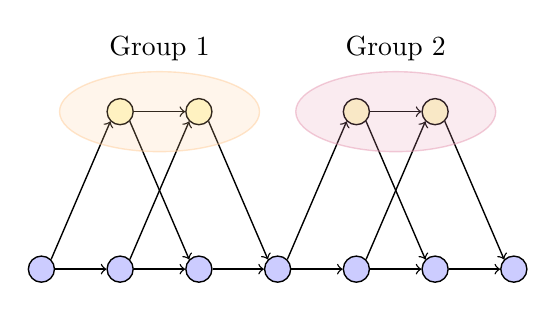
\begin{tikzpicture}
		\node[circle, fill=blue!20, line width=0.5pt, draw=black, minimum size=0.1in](one) at (0,0){};
		\node[circle, fill=blue!20, line width=0.5pt, draw=black, minimum size=0.1in](two) at (1,0){}; 
		\node[circle, fill=blue!20, line width=0.5pt, draw=black, minimum size=0.1in](three) at (2,0){};
		\node[circle, fill=blue!20, line width=0.5pt, draw=black, minimum size=0.1in](four) at (3,0){};
		\node[circle, fill=blue!20, line width=0.5pt, draw=black, minimum size=0.1in](five) at (4,0){};
		\node[circle, fill=blue!20, line width=0.5pt, draw=black, minimum size=0.1in](six) at (5,0){};
		\node[circle, fill=blue!20, line width=0.5pt, draw=black, minimum size=0.1in](seven) at (6,0){};
		\node[circle, fill=yellow!20, line width=0.5pt, draw=black, minimum size=0.1in](eight) at (1,2){};
		\node[circle, fill=yellow!20, line width=0.5pt, draw=black, minimum size=0.1in](nine) at (2,2){};
		\node[circle, fill=yellow!20, line width=0.5pt, draw=black, minimum size=0.1in](ten) at (4,2){}; 
		\node[circle, fill=yellow!20, line width=0.5pt, draw=black, minimum size=0.1in](eleven) at (5,2){}; 
		\draw [->, line width=0.5pt] (one.east) -- (two.west);
		\draw [->, line width=0.5pt] (two.east) -- (three.west);
		\draw [->, line width=0.5pt] (three.east) -- (four.west);
		\draw [->, line width=0.5pt] (four.east) -- (five.west);
		\draw [->, line width=0.5pt] (five.east) -- (six.west);
		\draw [->, line width=0.5pt] (six.east) -- (seven.west);
		\draw [->, line width=0.5pt] (one.north east) -- (eight.south west);
		\draw [->, line width=0.5pt] (two.north east) -- (nine.south west);
		\draw [->, line width=0.5pt] (four.north east) -- (ten.south west);
		\draw [->, line width=0.5pt] (five.north east) -- (eleven.south west);
		\draw [->, line width=0.5pt] (eight.south east) -- (three.north west);
		\draw [->, line width=0.5pt] (nine.south east) -- (four.north west);
		\draw [->, line width=0.5pt] (ten.south east) -- (six.north west);
		\draw [->, line width=0.5pt] (eleven.south east) -- (seven.north west);
		\draw [->, line width=0.5pt] (eight.east) -- (nine.west);
		\draw [->, line width=0.5pt] (ten.east) -- (eleven.west); 
		\node[ellipse, fill opacity=0.2, draw opacity=0.5, line width=0.5pt, draw=orange!40,fill=orange!40, minimum height=0.4in, minimum width=1in, label=Group 1](group1) at (1.5,2){};
		\node[ellipse, fill opacity=0.2, draw opacity=0.5, line width=0.5pt, draw=purple!40,fill=purple!40,  minimum height=0.4in, minimum width=1in, label=Group 2](group2) at (4.5,2){};
	\end{tikzpicture}
	\caption{Example of groups in a network flow graph.}
	\label{fig:groups}
\end{figure}
\begin{figure}
\centering
	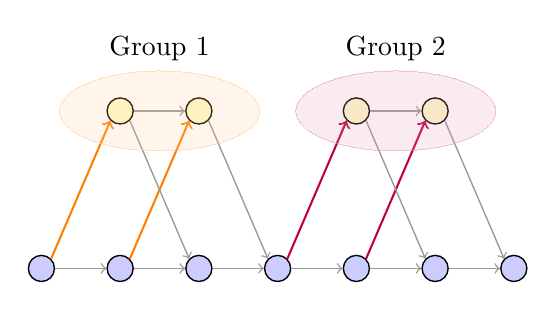
\begin{tikzpicture}
		\node[circle, fill=blue!20, line width=0.5pt, draw=black, minimum size=0.1in](one) at (0,0){};
		\node[circle, fill=blue!20, line width=0.5pt, draw=black, minimum size=0.1in](two) at (1,0){}; 
		\node[circle, fill=blue!20, line width=0.5pt, draw=black, minimum size=0.1in](three) at (2,0){};
		\node[circle, fill=blue!20, line width=0.5pt, draw=black, minimum size=0.1in](four) at (3,0){};
		\node[circle, fill=blue!20, line width=0.5pt, draw=black, minimum size=0.1in](five) at (4,0){};
		\node[circle, fill=blue!20, line width=0.5pt, draw=black, minimum size=0.1in](six) at (5,0){};
		\node[circle, fill=blue!20, line width=0.5pt, draw=black, minimum size=0.1in](seven) at (6,0){};
		\node[circle, fill=yellow!20, line width=0.5pt, draw=black, minimum size=0.1in](eight) at (1,2){};
		\node[circle, fill=yellow!20, line width=0.5pt, draw=black, minimum size=0.1in](nine) at (2,2){};
		\node[circle, fill=yellow!20, line width=0.5pt, draw=black, minimum size=0.1in](ten) at (4,2){}; 
		\node[circle, fill=yellow!20, line width=0.5pt, draw=black, minimum size=0.1in](eleven) at (5,2){}; 
		\draw [->, line width=0.5pt,color=black!40] (one.east) -- (two.west);
		\draw [->, line width=0.5pt,color=black!40] (two.east) -- (three.west);
		\draw [->, line width=0.5pt,color=black!40] (three.east) -- (four.west);
		\draw [->, line width=0.5pt,color=black!40] (four.east) -- (five.west);
		\draw [->, line width=0.5pt,color=black!40] (five.east) -- (six.west);
		\draw [->, line width=0.5pt,color=black!40] (six.east) -- (seven.west);
		\draw [->, color=orange, line width=0.75pt] (one.north east) -- (eight.south west);
		\draw [->, color=orange, line width=0.75pt] (two.north east) -- (nine.south west);
		\draw [->, color=purple, line width=0.75pt] (four.north east) -- (ten.south west);
		\draw [->, color=purple, line width=0.75pt] (five.north east) -- (eleven.south west);
		\draw [->, line width=0.5pt,color=black!40] (eight.south east) -- (three.north west);
		\draw [->, line width=0.5pt,color=black!40] (nine.south east) -- (four.north west);
		\draw [->, line width=0.5pt,color=black!40] (ten.south east) -- (six.north west);
		\draw [->, line width=0.5pt,color=black!40] (eleven.south east) -- (seven.north west);
		\draw [->, line width=0.5pt,color=black!40] (eight.east) -- (nine.west);
		\draw [->, line width=0.5pt,color=black!40] (ten.east) -- (eleven.west); 
		\node[ellipse, line width=0pt, draw opacity=0.5, fill opacity=0.2, fill=purple!40, draw=purple!40, minimum height=0.4in, minimum width=1in, label=Group 2](group2) at (4.5,2){};
		\node[ellipse, line width=0pt, draw opacity=0.5, fill opacity=0.2, fill=orange!40, draw=orange!40, minimum height=0.4in, minimum width=1in, label=Group 1](group1) at (1.5,2){};
	\end{tikzpicture}
	\caption{Incoming group edges.}
	\label{fig:groupedEdges} 
\end{figure} 
Let $\mathbf{x}$ be the edge weights as before and $\mathbf{c}_g$ be an $n_G \times 1$ vector where the $i^{\text{th}}$ element gives the group flow for group $i$. The group flow is then computed as 
\begin{align}\label{eqn:cGroupFlow}
	B\mathbf{x} = \mathbf{c}_g
\end{align}
But the group flow is required to be one at most to avoid connection thrashing.  This is expressed by the inequality given in equation (\ref{eqn:cGroupFlow}).
\begin{align}\label{eqn:cGroupFlow}
	Bx \le \mathbf{1}.
\end{align}
Similarly to (\ref{eqn:cFlow2}), equation (\ref{eqn:cGroupFlow}) can also be expressed in terms of $\mathbf{y}$ with appropriate zero padding as
\begin{equation}\label{eqn:cGroupFlow2}
	\begin{aligned}
		\begin{bmatrix} B & 0\end{bmatrix} \mathbf{y} &= \tilde{B}\mathbf{y} = \mathbf{1} \\
	\end{aligned}
\end{equation}
\subsection{Section Summary} In summary, the bus charge problem can be formulated as a graph with nodes and edges, where charge plans are encoded as a path with unit edge weights. The charge problem aims to find a feasible path which minimizes the cost of power. Feasibility is defined through a set of net-flow and group-flow constraints. Net-flow constraints are encoded through an adjacency matrix and enforce both the conservation and total number of chargers. The group-flow constraints prevent connection thrashing and limit to one the number of simultaneous charger-to-bus connections. 
\begin{figure}
\centering
	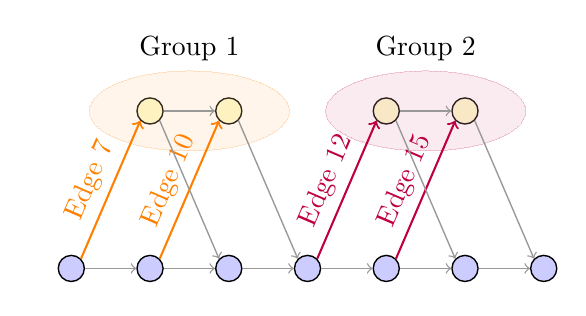
\begin{tikzpicture}
		\node[circle, fill=blue!20, line width=0.5pt, draw=black, minimum size=0.1in](one) at (0,0){};
		\node[circle, fill=blue!20, line width=0.5pt, draw=black, minimum size=0.1in](two) at (1,0){}; 
		\node[circle, fill=blue!20, line width=0.5pt, draw=black, minimum size=0.1in](three) at (2,0){};
		\node[circle, fill=blue!20, line width=0.5pt, draw=black, minimum size=0.1in](four) at (3,0){};
		\node[circle, fill=blue!20, line width=0.5pt, draw=black, minimum size=0.1in](five) at (4,0){};
		\node[circle, fill=blue!20, line width=0.5pt, draw=black, minimum size=0.1in](six) at (5,0){};
		\node[circle, fill=blue!20, line width=0.5pt, draw=black, minimum size=0.1in](seven) at (6,0){};
		\node[circle, fill=yellow!20, line width=0.5pt, draw=black, minimum size=0.1in](eight) at (1,2){};
		\node[circle, fill=yellow!20, line width=0.5pt, draw=black, minimum size=0.1in](nine) at (2,2){};
		\node[circle, fill=yellow!20, line width=0.5pt, draw=black, minimum size=0.1in](ten) at (4,2){}; 
		\node[circle, fill=yellow!20, line width=0.5pt, draw=black, minimum size=0.1in](eleven) at (5,2){}; 
		\node[ellipse, line width=0pt, draw opacity=0.5, fill opacity=0.2, fill=purple!40, draw=purple!40, minimum height=0.4in, minimum width=1in, label=Group 2](group2) at (4.5,2){};
		\node[ellipse, line width=0pt, draw opacity=0.5, fill opacity=0.2, fill=orange!40, draw=orange!40, minimum height=0.4in, minimum width=1in, label=Group 1](group1) at (1.5,2){};
		\draw [->, line width=0.5pt,color=black!40] (one.east) -- (two.west);
		\draw [->, line width=0.5pt,color=black!40] (two.east) -- (three.west);
		\draw [->, line width=0.5pt,color=black!40] (three.east) -- (four.west);
		\draw [->, line width=0.5pt,color=black!40] (four.east) -- (five.west);
		\draw [->, line width=0.5pt,color=black!40] (five.east) -- (six.west);
		\draw [->, line width=0.5pt,color=black!40] (six.east) -- (seven.west);
		\draw [->, color=orange, line width=0.75pt] (one.north east) -- node[sloped, anchor=center, above, text width=2.5cm, align=center]{Edge 7}(eight.south west);
		\draw [->, color=orange, line width=0.75pt] (two.north east) -- node[sloped, anchor=center, above, text width=2.5cm, align=center]{Edge 10}(nine.south west);
		\draw [->, color=purple, line width=0.75pt] (four.north east) -- node[sloped, anchor=center, above, text width=2.5cm, align=center]{Edge 12}(ten.south west);
		\draw [->, color=purple, line width=0.75pt] (five.north east) -- node[sloped, anchor=center, above, text width=2.5cm, align=center]{Edge 15}(eleven.south west);
		\draw [->, line width=0.5pt,color=black!40] (eight.south east) -- (three.north west);
		\draw [->, line width=0.5pt,color=black!40] (nine.south east) -- (four.north west);
		\draw [->, line width=0.5pt,color=black!40] (ten.south east) -- (six.north west);
		\draw [->, line width=0.5pt,color=black!40] (eleven.south east) -- (seven.north west);
		\draw [->, line width=0.5pt,color=black!40] (eight.east) -- (nine.west);
		\draw [->, line width=0.5pt,color=black!40] (ten.east) -- (eleven.west); 
	\end{tikzpicture}
	\caption{Connect edge example for groups.}
	\label{fig:groupEdges} 
\end{figure} 

\section{Battery State of Charge}
The state of charge (SOC) is influenced in three ways; initial conditions, discharge events, and traversing charge nodes (as shown in figure \ref{fig:edgeTypes}).  There are SOC variables for each node representing an available bus, where the SOC value for the ith bus at SOC index j is denoted as $d_{i,j}$ as shown in figure \ref{fig:socDiagram}.  Note, there only needs be SOC variables for time indices where buses are available to charge and $d_{i,j}$ does not generally correspond to the charge at \textit{time interval} j.  All other timesteps are deterministic and need not be computed.

\begin{figure}
	\centering
	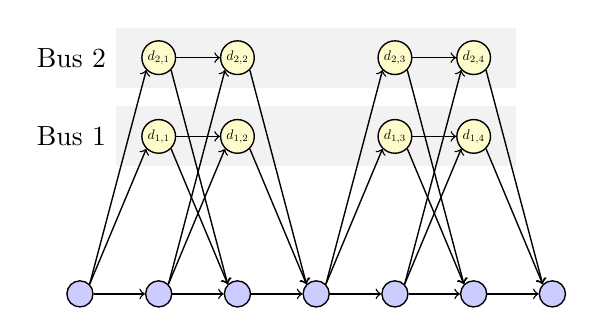
\begin{tikzpicture} 

		\node[rectangle, fill=gray!10, minimum width=2in, minimum height=.3in,label=left:Bus 2](bus2Box) at (3,3){};
		\node[rectangle, fill=gray!10, minimum width=2in, minimum height=.3in,label=left:Bus 1](bus1Box) at (3,2){};

		\node[circle, fill=blue!20, line width=0.5pt, draw=black, minimum size=0.1in](one) at (0,0){};
		\node[circle, fill=blue!20, line width=0.5pt, draw=black, minimum size=0.1in](two) at (1,0){}; 
		\node[circle, fill=blue!20, line width=0.5pt, draw=black, minimum size=0.1in](three) at (2,0){};
		\node[circle, fill=blue!20, line width=0.5pt, draw=black, minimum size=0.1in](four) at (3,0){};
		\node[circle, fill=blue!20, line width=0.5pt, draw=black, minimum size=0.1in](five) at (4,0){};
		\node[circle, fill=blue!20, line width=0.5pt, draw=black, minimum size=0.1in](six) at (5,0){};
		\node[circle, fill=blue!20, line width=0.5pt, draw=black, minimum size=0.1in](seven) at (6,0){};
		
		\node[circle, fill=yellow!20, line width=0.5pt, draw=black, minimum size=0.1in, inner sep=1pt](eight) at (1,2){\scalebox{0.5}{$d_{1,1}$}};
		\node[circle, fill=yellow!20, line width=0.5pt, draw=black, minimum size=0.1in, inner sep=1pt](nine) at (2,2){\scalebox{0.5}{$d_{1,2}$}};
		\node[circle, fill=yellow!20, line width=0.5pt, draw=black, minimum size=0.1in, inner sep=1pt](ten) at (4,2){\scalebox{0.5}{$d_{1,3}$}}; 
		\node[circle, fill=yellow!20, line width=0.5pt, draw=black, minimum size=0.1in, inner sep=1pt](eleven) at (5,2){\scalebox{0.5}{$d_{1,4}$}}; 

		\node[circle, fill=yellow!20, line width=0.5pt, draw=black, minimum size=0.1in, inner sep=1pt](twelve) at (1,3){\scalebox{0.5}{$d_{2,1}$}};
		\node[circle, fill=yellow!20, line width=0.5pt, draw=black, minimum size=0.1in, inner sep=1pt](thirteen) at (2,3){\scalebox{0.5}{$d_{2,2}$}};
		\node[circle, fill=yellow!20, line width=0.5pt, draw=black, minimum size=0.1in, inner sep=1pt](fourteen) at (4,3){\scalebox{0.5}{$d_{2,3}$}}; 
		\node[circle, fill=yellow!20, line width=0.5pt, draw=black, minimum size=0.1in, inner sep=1pt](fifteen) at (5,3){\scalebox{0.5}{$d_{2,4}$}}; 

		\draw [->, line width=0.5pt] (one.east) -- (two.west);
		\draw [->, line width=0.5pt] (two.east) -- (three.west);
		\draw [->, line width=0.5pt] (three.east) -- (four.west);
		\draw [->, line width=0.5pt] (four.east) -- (five.west);
		\draw [->, line width=0.5pt] (five.east) -- (six.west);
		\draw [->, line width=0.5pt] (six.east) -- (seven.west);

		\draw [->, line width=0.5pt] (one.north east) -- (eight.south west);
		\draw [->, line width=0.5pt] (two.north east) -- (nine.south west);
		\draw [->, line width=0.5pt] (four.north east) -- (ten.south west);
		\draw [->, line width=0.5pt] (five.north east) -- (eleven.south west);
		\draw [->, line width=0.5pt] (eight.south east) -- (three.north west);
		\draw [->, line width=0.5pt] (nine.south east) -- (four.north west);
		\draw [->, line width=0.5pt] (ten.south east) -- (six.north west);
		\draw [->, line width=0.5pt] (eleven.south east) -- (seven.north west);
		\draw [->, line width=0.5pt] (eight.east) -- (nine.west);
		\draw [->, line width=0.5pt] (ten.east) -- (eleven.west); 

		\draw [->, line width=0.5pt] (one.north east) -- (twelve.south west);
		\draw [->, line width=0.5pt] (two.north east) -- (thirteen.south west);
		\draw [->, line width=0.5pt] (four.north east) -- (fourteen.south west);
		\draw [->, line width=0.5pt] (five.north east) -- (fifteen.south west);
		\draw [->, line width=0.5pt] (twelve.south east) -- (three.north west);
		\draw [->, line width=0.5pt] (thirteen.south east) -- (four.north west);
		\draw [->, line width=0.5pt] (fourteen.south east) -- (six.north west);
		\draw [->, line width=0.5pt] (fifteen.south east) -- (seven.north west);
		\draw [->, line width=0.5pt] (twelve.east) -- (thirteen.west);
		\draw [->, line width=0.5pt] (fourteen.east) -- (fifteen.west); 

	\end{tikzpicture}
	\caption{SOC indicators}
	\label{fig:socDiagram}
\end{figure}
\par When charging, the change in SOC associated with the ith bus at the jth charge edge is denoted $g_{i,j}$. Again, note that j is \textit{not} indicative of a time interval, rather it gives the \textit{index} of the \textit{charge edge} in use as shown in figure \ref{fig:dSocDiagram}.
\begin{figure}
	\centering
	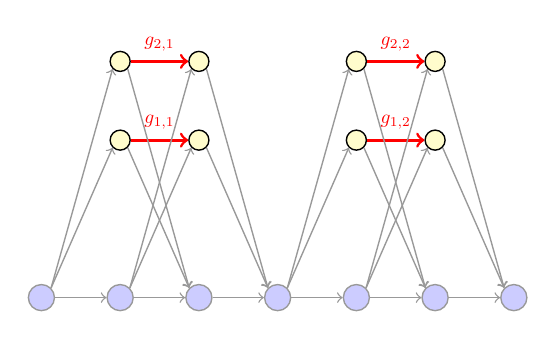
\begin{tikzpicture} 

		\node[circle, fill=blue!20, line width=0.5pt, draw=black!40, minimum size=0.1in](one) at (0,0){};
		\node[circle, fill=blue!20, line width=0.5pt, draw=black!40, minimum size=0.1in](two) at (1,0){}; 
		\node[circle, fill=blue!20, line width=0.5pt, draw=black!40, minimum size=0.1in](three) at (2,0){};
		\node[circle, fill=blue!20, line width=0.5pt, draw=black!40, minimum size=0.1in](four) at (3,0){};
		\node[circle, fill=blue!20, line width=0.5pt, draw=black!40, minimum size=0.1in](five) at (4,0){};
		\node[circle, fill=blue!20, line width=0.5pt, draw=black!40, minimum size=0.1in](six) at (5,0){};
		\node[circle, fill=blue!20, line width=0.5pt, draw=black!40, minimum size=0.1in](seven) at (6,0){};
		
		\node[circle, fill=yellow!20, line width=0.5pt, draw=black, minimum size=0.1in, inner sep=1pt](eight) at (1,2){};
		\node[circle, fill=yellow!20, line width=0.5pt, draw=black, minimum size=0.1in, inner sep=1pt](nine) at (2,2){};
		\node[circle, fill=yellow!20, line width=0.5pt, draw=black, minimum size=0.1in, inner sep=1pt](ten) at (4,2){};
		\node[circle, fill=yellow!20, line width=0.5pt, draw=black, minimum size=0.1in, inner sep=1pt](eleven) at (5,2){};

		\node[circle, fill=yellow!20, line width=0.5pt, draw=black, minimum size=0.1in, inner sep=1pt](twelve) at (1,3){};
		\node[circle, fill=yellow!20, line width=0.5pt, draw=black, minimum size=0.1in, inner sep=1pt](thirteen) at (2,3){};
		\node[circle, fill=yellow!20, line width=0.5pt, draw=black, minimum size=0.1in, inner sep=1pt](fourteen) at (4,3){};
		\node[circle, fill=yellow!20, line width=0.5pt, draw=black, minimum size=0.1in, inner sep=1pt](fifteen) at (5,3){};

		\draw [->, line width=0.5pt, color=black!40] (one.east) -- (two.west);
		\draw [->, line width=0.5pt, color=black!40] (two.east) -- (three.west);
		\draw [->, line width=0.5pt, color=black!40] (three.east) -- (four.west);
		\draw [->, line width=0.5pt, color=black!40] (four.east) -- (five.west);
		\draw [->, line width=0.5pt, color=black!40] (five.east) -- (six.west);
		\draw [->, line width=0.5pt, color=black!40] (six.east) -- (seven.west);

		\draw [->, line width=0.5pt, color=black!40] (one.north east) -- (eight.south west);
		\draw [->, line width=0.5pt, color=black!40] (two.north east) -- (nine.south west);
		\draw [->, line width=0.5pt, color=black!40] (four.north east) -- (ten.south west);
		\draw [->, line width=0.5pt, color=black!40] (five.north east) -- (eleven.south west);
		\draw [->, line width=0.5pt, color=black!40] (eight.south east) -- (three.north west);
		\draw [->, line width=0.5pt, color=black!40] (nine.south east) -- (four.north west);
		\draw [->, line width=0.5pt, color=black!40] (ten.south east) -- (six.north west);
		\draw [->, line width=0.5pt, color=black!40] (eleven.south east) -- (seven.north west);
		\draw [->, line width=1pt, color=red] (eight.east) -- node[above]{\scalebox{0.7}{$g_{1,1}$}}(nine.west);
		\draw [->, line width=1pt, color=red] (ten.east) -- node[above]{\scalebox{0.7}{$g_{1,2}$}}(eleven.west); 

		\draw [->, line width=0.5pt, color=black!40] (one.north east) -- (twelve.south west);
		\draw [->, line width=0.5pt, color=black!40] (two.north east) -- (thirteen.south west);
		\draw [->, line width=0.5pt, color=black!40] (four.north east) -- (fourteen.south west);
		\draw [->, line width=0.5pt, color=black!40] (five.north east) -- (fifteen.south west);
		\draw [->, line width=0.5pt, color=black!40] (twelve.south east) -- (three.north west);
		\draw [->, line width=0.5pt, color=black!40] (thirteen.south east) -- (four.north west);
		\draw [->, line width=0.5pt, color=black!40] (fourteen.south east) -- (six.north west);
		\draw [->, line width=0.5pt, color=black!40] (fifteen.south east) -- (seven.north west);
		\draw [->, line width=1pt, color=red] (twelve.east) -- node[above]{\scalebox{0.7}{$g_{2,1}$}}(thirteen.west);
		\draw [->, line width=1pt, color=red] (fourteen.east) -- node[above]{\scalebox{0.7}{$g_{2,2}$}}(fifteen.west); 

	\end{tikzpicture}
	\caption{Depiction of which edges increase SOC for the single rate case}
	\label{fig:dSocDiagram}
\end{figure}
\par An additional contribution this paper gives is the addition of multi-rate charging.  This adapts the basic methodology to incorporate additional charge edges and $g_{i,j}$ variables.  Under this methodology, the graph given in figure \ref{fig:groups} would be modified to reflect figure \ref{fig:multiRateChargeEdges}, where $g_{i,j,k}$ represents the ith bus at charge instance j and charge rate k.
\begin{figure}
	\centering
	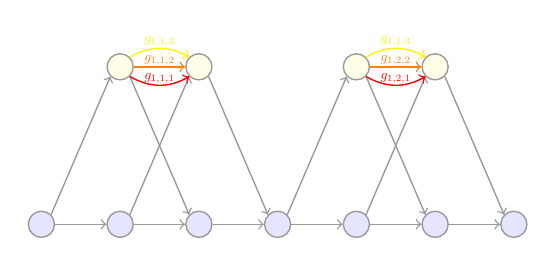
\begin{tikzpicture}[->, line width=0.5pt]
		\node[circle, fill=blue!10, draw=black!40,line width=0.5pt, minimum size=0.1in](one) at (0,0){};
		\node[circle, fill=blue!10, draw=black!40,line width=0.5pt, minimum size=0.1in](two) at (1,0){}; 
		\node[circle, fill=blue!10, draw=black!40,line width=0.5pt, minimum size=0.1in](three) at (2,0){};
		\node[circle, fill=blue!10, draw=black!40,line width=0.5pt, minimum size=0.1in](four) at (3,0){};
		\node[circle, fill=blue!10, draw=black!40,line width=0.5pt, minimum size=0.1in](five) at (4,0){};
		\node[circle, fill=blue!10, draw=black!40,line width=0.5pt, minimum size=0.1in](six) at (5,0){};
		\node[circle, fill=blue!10, draw=black!40,line width=0.5pt, minimum size=0.1in](seven) at (6,0){};
		\node[circle, fill=yellow!10, draw=black!40,line width=0.5pt, minimum size=0.1in](eight) at (1,2){};
		\node[circle, fill=yellow!10, draw=black!40,line width=0.5pt, minimum size=0.1in](nine) at (2,2){};
		\node[circle, fill=yellow!10, draw=black!40,line width=0.5pt, minimum size=0.1in](ten) at (4,2){}; 
		\node[circle, fill=yellow!10, draw=black!40,line width=0.5pt, minimum size=0.1in](eleven) at (5,2){}; 
		\draw [line width=0.5pt,color=black!40] (one.east) -- (two.west);
		\draw [line width=0.5pt,color=black!40] (two.east) -- (three.west);
		\draw [line width=0.5pt,color=black!40] (three.east) -- (four.west);
		\draw [line width=0.5pt,color=black!40] (four.east) -- (five.west);
		\draw [line width=0.5pt,color=black!40] (five.east) -- (six.west);
		\draw [line width=0.5pt,color=black!40] (six.east) -- (seven.west);
		\draw [line width=0.5pt,color=black!40] (one.north east) -- (eight.south west);
		\draw [line width=0.5pt,color=black!40] (two.north east) -- (nine.south west);
		\draw [line width=0.5pt,color=black!40] (four.north east) -- (ten.south west);
		\draw [line width=0.5pt,color=black!40] (five.north east) -- (eleven.south west);
		\draw [line width=0.5pt,color=black!40] (eight.south east) -- (three.north west);
		\draw [line width=0.5pt,color=black!40] (nine.south east) -- (four.north west);
		\draw [line width=0.5pt,color=black!40] (ten.south east) -- (six.north west);
		\draw [line width=0.5pt,color=black!40] (eleven.south east) -- (seven.north west);

		\draw [color=yellow,-,line width=0.5pt] (eight.north east) edge[->,bend left]node[above=-3pt]{\scalebox{0.5}{$g_{1,1,3}$}}(nine.north west);
		\draw [color=orange,line width=0.5pt] (eight.east) -- node[above=-3pt]{\scalebox{0.5}{$g_{1,1,2}$}}(nine.west);
		\draw [color=red,-,line width=0.5pt] (eight.south east) edge[->, bend right]node[above=-3pt]{\scalebox{0.5}{$g_{1,1,1}$}}(nine.south west);

		\draw [color=yellow,-, line width=0.5pt] (ten.north east) edge[->, bend left]node[above=-3pt]{\scalebox{0.5}{$g_{1,1,3}$}}(eleven.north west);
		\draw [color=orange,line width=0.5pt] (ten.east) -- node[above=-3pt]{\scalebox{0.5}{$g_{1,2,2}$}}(eleven.west); 
		\draw [color=red,-, line width=0.5pt] (ten.south east) edge[->, bend right]node[above=-3pt]{\scalebox{0.5}{$g_{1,2,1}$}}(eleven.south west);
	\end{tikzpicture}
	\caption{Multi-Rate Charging}
	\label{fig:multiRateChargeEdges}
\end{figure}
\par To model the effect of charging on a battery state of charge, we adopt the Constant Current Constant Voltage (CCCV) model as derived in \cite{whitaker_network_2021} which gives
\begin{align}
	s_{k+1} = \bar{a}_ls_k - \bar{b}_lM 
\end{align}
Where $s_k$ is the charge of a battery at time $k$, $\bar{a}_l$ is a charge rate dependent, experimentally determined value, $\bar{b_l} = \bar{a_l} - 1$, and $M$ is the maximum capacity of the battery in kWh.  
\par Recall how $g$ represented the change in state of charge of the battery in kWh.  This allows us to express $s_{k+1}$ in terms of 
\begin{align}
	s_{k+1} = s_k + g_{\pi_g(m,k,l)}
\end{align}
where $\pi_g(m,k,l)$ represents the index of $g$ for bus $m$ at time index $k$ for charge rate $l$.  These two equations imply that
\begin{equation}
\begin{aligned}
	s_k + g_{\pi_g(m,k,l)} &= \bar{a}_ls_k - \bar{b}_lM \\
\Rightarrow g_{\pi_g(m,k,l)} &=  \bar{a}_ls_k - s_k - \bar{b}_lM \\
\Rightarrow g_{\pi_g(m,k,l)} &=  s_k(\bar{a}_l - 1) - \bar{b}_lM.
\end{aligned}
\end{equation}
But the state of charges for bus $m$ are given in terms of $d_{i,j}$.  If we let $d_{i,j} = \pi_d(i,k,l)$, then the final expression for $g$ becomes
\begin{align}\label{eqn:g}
	g_{\pi_g(m,k,l)} = d_{\pi_d(m,k,l)}(\bar{a}_l - 1) - \bar{b}_lM.
\end{align}
Note, \ref{eqn:g} is only valid when the bus is charging and must be tempered with additional constraints to account for the non-charging case.
\par To handle the two cases, we express the cases for charging (equation \ref{eqn:g} and non-charging ($g=0$) as  
\begin{equation}
\begin{aligned}
	g_{\pi_g(m,k,l)}  &= d_{\pi_d(m,k,l)}(\bar{a}_l - 1) - \bar{b}_lM \\
	g_{\pi_g(m,k,l)} &= 0.
\end{aligned}
\end{equation}
which also implies that
\begin{equation}\label{eqn:gTwoConst}
\begin{aligned}
	g_{\pi_g(m,k,l)}  &\le d_{\pi_d(m,k,l)}(\bar{a}_l - 1) - \bar{b}_lM \\
	g_{\pi_g(m,k,l)}  &\ge d_{\pi_d(m,k,l)}(\bar{a}_l - 1) - \bar{b}_lM \\
	g_{\pi_g(m,k,l)} &\le 0 \\
	g_{\pi_g(m,k,l)} &\ge 0.
\end{aligned}
\end{equation}
Next, let $x_{\pi_x(m,k,l)}$ be the index of the edge corresponding to $g_{\pi_g(m,k,l)}$.  A switch between the two constarints expressed in equation \ref{eqn:gTwoConst} can be constructed using the \textit{big M} technique.  This modifies equation \ref{eqn:gTwoConst} such that
\begin{equation}\label{eqn:gBigM}
	\begin{aligned}
		g_{\pi_g(m,k,l)}  &\le d_{\pi_d(m,k,l)}(\bar{a}_l - 1) - \bar{b}_lM - M(1 - x_{\pi_x(m,k,l)})\\
		g_{\pi_g(m,k,l)}  &\ge d_{\pi_d(m,k,l)}(\bar{a}_l - 1) - \bar{b}_lM \\
		g_{\pi_g(m,k,l)} &\le 0 + Mx_{\pi_x(m,k,l)})\\
		g_{\pi_g(m,k,l)} &\ge 0.  
	\end{aligned}
\end{equation}
Note that as expressed, when the charge edge is active (i.e. $x_{\pi_x(m,k,l)} = 1$), then 
\begin{equation}
	\begin{aligned}
		\color{blue}{g_{\pi_g(m,k,l)}}  &\color{blue}{\le d_{\pi_d(m,k,l)}(\bar{a}_l - 1) - \bar{b}_lM} \\
		\color{blue}{g_{\pi_g(m,k,l)}}  &\color{blue}{\ge d_{\pi_d(m,k,l)}(\bar{a}_l - 1) - \bar{b}_lM} \\
		\color{red}{g_{\pi_g(m,k,l)}} & \color{red}{\le M} \\
		\color{red}{g_{\pi_g(m,k,l)}} & \color{red}{\ge 0}.  
	\end{aligned}
\end{equation}
Bus as $g$ can never exceed the charge capacity of the battery, the bottom two constraints are inactive and $g$ is both less than or greater than equation \ref{eqn:g}, making it equal.  When the edge is inactive, or $x_{\pi_x(m,k,l)} = 0$, equation \ref{eqn:gBigM} becomes
\begin{equation}
	\begin{aligned}
		\color{red}{g_{\pi_g(m,k,l)}}  &\color{red}{\le d_{\pi_d(m,k,l)}(\bar{a}_l - 1) - \bar{b}_lM - M} \\
		\color{red}{g_{\pi_g(m,k,l)}}  &\color{red}{\ge d_{\pi_d(m,k,l)}(\bar{a}_l - 1) - \bar{b}_lM} \\
		\color{blue}{g_{\pi_g(m,k,l)}} &\color{blue}{\le 0} \\
		\color{blue}{g_{\pi_g(m,k,l)}} &\color{blue}{\ge 0}.  
	\end{aligned}
\end{equation}
where the top two constraints become inactive and $g$ is both less than and greater than 0, making it equal.
Hence, these constraints can be expressed in linear form as
\begin{equation}\label{eqn:chargeConstraints}
	\begin{aligned} 
		-g_{m,k,l} + d_{m,k,l}(\bar{a}_l - 1) + x_{m,k,l} &\le M(\bar{b}_l + 1) \\
		 g_{m,k,l} - d_{m,k,l}(\bar{a}_l - 1)  &\le  - \bar{b}_lM \\
		 g_{m,k,l} - Mx_{m,k,l} &\le 0 \\
		-g_{m,k,l} &\le 0.  
	\end{aligned}
\end{equation}
\par The constraints for state of charge are circumstantially dependent. Each $d_{m,k,l}$ must be defined by a set of constraints which are defined by either initial conditions, previous graphs, route discharge, or $g_{m,k,l}$ variables.
\par Initial conditions and previous graphs are straight forward.  Initial conditions are given as an equality constraint.  For example, if $d_0$ was initialized to 80 kWh, the constraint would be $d_0 = 80$.  To initialize to the value of a previous graph, use an equality constraint.  
\par Suppose we modeled early morning and day-time operations and had two corresponding graphs. The final node of graph one would be equivalent to the first node of graph two in the temporal sense and the corresponding $d_{m,l,k}$ values would also be equated as $d_{\text{Graph 1}} - d_{\text{Graph 2}} = 0$.
\par $d_{m,l,k}$ values corresponding to available charge times are expressed as a sum of $g_{m,k,l}$ values given in equation \ref{eqn:chargeConstraints} such that
\begin{align*}
	d_{m,k + 1} = d_{m,k} + \sum_l{g_{m,k,l}}
\end{align*}
or as given in linear form,
\begin{align}
	d_{m,k+1} - d_{m,k} - \sum_l{g_{m,k,l}} = 0.
\end{align}
\par The final case deals with battery discharge over a route.  As seen in figure \ref{fig:delta}, discharge values, also refered to as $\delta$ represent the power expenditure overa route.  This expenditure is modeled as a withdrawel from the resevour in a battery and was calibrated from data received from the Utah Transit Authority.  In figure \ref{fig:delta}, the SOC constraints corresponding to $\delta_1$ would be as follow:
\begin{align*}
	d_{1,3} = d_{1,2} - \delta_1
\end{align*}
or in linear form,
\begin{align}
	d_{1,2} - d_{1,3} = \delta_1.
\end{align}
\begin{figure}
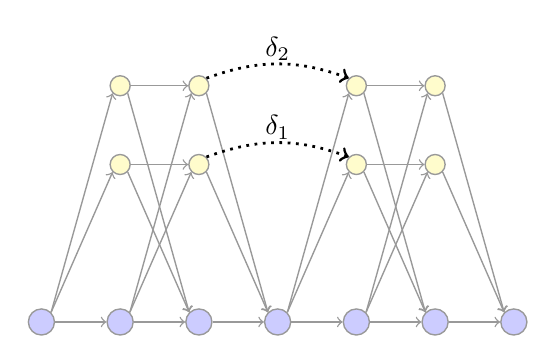
\begin{tikzpicture}
	\node[circle, fill=blue!20, line width=0.5pt, draw=black!40, minimum size=0.1in](one) at (0,0){};
	\node[circle, fill=blue!20, line width=0.5pt, draw=black!40, minimum size=0.1in](two) at (1,0){}; 
	\node[circle, fill=blue!20, line width=0.5pt, draw=black!40, minimum size=0.1in](three) at (2,0){};
	\node[circle, fill=blue!20, line width=0.5pt, draw=black!40, minimum size=0.1in](four) at (3,0){};
	\node[circle, fill=blue!20, line width=0.5pt, draw=black!40, minimum size=0.1in](five) at (4,0){};
	\node[circle, fill=blue!20, line width=0.5pt, draw=black!40, minimum size=0.1in](six) at (5,0){};
	\node[circle, fill=blue!20, line width=0.5pt, draw=black!40, minimum size=0.1in](seven) at (6,0){};
	
	\node[circle, fill=yellow!20, line width=0.5pt, draw=black!40, minimum size=0.1in, inner sep=1pt](eight) at (1,2){};
	\node[circle, fill=yellow!20, line width=0.5pt, draw=black!40, minimum size=0.1in, inner sep=1pt](nine) at (2,2){};
	\node[circle, fill=yellow!20, line width=0.5pt, draw=black!40, minimum size=0.1in, inner sep=1pt](ten) at (4,2){};
	\node[circle, fill=yellow!20, line width=0.5pt, draw=black!40, minimum size=0.1in, inner sep=1pt](eleven) at (5,2){};

	\node[circle, fill=yellow!20, line width=0.5pt, draw=black!40, minimum size=0.1in, inner sep=1pt](twelve) at (1,3){};
	\node[circle, fill=yellow!20, line width=0.5pt, draw=black!40, minimum size=0.1in, inner sep=1pt](thirteen) at (2,3){};
	\node[circle, fill=yellow!20, line width=0.5pt, draw=black!40, minimum size=0.1in, inner sep=1pt](fourteen) at (4,3){};
	\node[circle, fill=yellow!20, line width=0.5pt, draw=black!40, minimum size=0.1in, inner sep=1pt](fifteen) at (5,3){};

	\draw [->, line width=0.5pt, color=black!40] (one.east) -- (two.west);
	\draw [->, line width=0.5pt, color=black!40] (two.east) -- (three.west);
	\draw [->, line width=0.5pt, color=black!40] (three.east) -- (four.west);
	\draw [->, line width=0.5pt, color=black!40] (four.east) -- (five.west);
	\draw [->, line width=0.5pt, color=black!40] (five.east) -- (six.west);
	\draw [->, line width=0.5pt, color=black!40] (six.east) -- (seven.west);

	\draw [->, line width=0.5pt, color=black!40] (one.north east) -- (eight.south west);
	\draw [->, line width=0.5pt, color=black!40] (two.north east) -- (nine.south west);
	\draw [->, line width=0.5pt, color=black!40] (four.north east) -- (ten.south west);
	\draw [->, line width=0.5pt, color=black!40] (five.north east) -- (eleven.south west);
	\draw [->, line width=0.5pt, color=black!40] (eight.south east) -- (three.north west);
	\draw [->, line width=0.5pt, color=black!40] (nine.south east) -- (four.north west);
	\draw [->, line width=0.5pt, color=black!40] (ten.south east) -- (six.north west);
	\draw [->, line width=0.5pt, color=black!40] (eleven.south east) -- (seven.north west);
	\draw [->, line width=0.5pt, color=black!40] (eight.east) -- (nine.west);
	\draw [->, line width=0.5pt, color=black!40] (ten.east) -- (eleven.west); 

	\draw [->, line width=0.5pt, color=black!40] (one.north east) -- (twelve.south west);
	\draw [->, line width=0.5pt, color=black!40] (two.north east) -- (thirteen.south west);
	\draw [->, line width=0.5pt, color=black!40] (four.north east) -- (fourteen.south west);
	\draw [->, line width=0.5pt, color=black!40] (five.north east) -- (fifteen.south west);
	\draw [->, line width=0.5pt, color=black!40] (twelve.south east) -- (three.north west);
	\draw [->, line width=0.5pt, color=black!40] (thirteen.south east) -- (four.north west);
	\draw [->, line width=0.5pt, color=black!40] (fourteen.south east) -- (six.north west);
	\draw [->, line width=0.5pt, color=black!40] (fifteen.south east) -- (seven.north west);
	\draw [->, line width=0.5pt, color=black!40] (twelve.east) -- (thirteen.west);
	\draw [->, line width=0.5pt, color=black!40] (fourteen.east) -- (fifteen.west); 
	\draw [dotted, color=black,-,line width=1pt] (nine.north east) edge[->,bend left=20pt]node[above=-2.5pt]{\scalebox{1}{$\delta_1$}}(ten.north west); 
	\draw [dotted, color=black,-,line width=1pt] (thirteen.north east) edge[->,bend left=20pt]node[above=-2.5pt]{\scalebox{1}{$\delta_2$}}(fourteen.north west); 
\end{tikzpicture}
	\caption{$\delta$ values for routes}
	\label{fig:delta}
\end{figure} 

\section{Multi-Graph Additions}
An additional contribution this work offers is the expansion to joint optimization of both night and day charging in a single optimization problem. Day and night operations differ in two aspects: number of chargers and bus availability. During the day, the buses can charge only at the charge station. The number of chargers in the station are limited, causing contention between buses. At night, each bus docks in a holding stall with one charger per stall, eliminating charger contention. Furthermore, nighttime charging is slow compred to daytime charing.  Our model uses different rates for day and night charging.
\par Bus availability also changes because buses do not leave their stalls at night. This simplifies the charge problem because buses are always available for charging. 
\par Equation (\ref{eqn:cFlow}) in section \ref{sec:net-flow} describes the net-flow constraints which constrain the number of chargers in the source and sink nodes. Because the number of chargers are different from night to day, a separate graph is used at each transition as shown in Fig.~\ref{fig:nightVsDayGraph}.
\par Each graph is connected by equating the appropriate SOC values.  Consider the multi-graph formulation given in Fig.~\ref{fig:nightVsDayConnected}.  The morning graph is related to the day graph because $d_{1,1}$ and $d_{2,1}$ represent the same SOC values as $d_{1,2}$ and $d_{2,2}$ respectively. The same applies for the day and night graphs, where $d_{1,5}$ and $d_{2,5}$ represent the SOC values for $d_{1,6}$ and $d_{2,6}$. This equality relationship can be expressed as an equality constraint where
\begin{align}
	\mathbf{d}_{\text{graph 1}} - \mathbf{d}_{\text{graph 2}} = \mathbf{0},,,,
\end{align}
or by 
\begin{align}\label{eqn:multiGraphConst}
	D_\text{multi-graph}\mathbf{y} = \mathbf{0},
\end{align}
where $D_\text{multi-graph}$ is an $\text{nBus} \times \text{nVar}$ matrix such that
\begin{align}
	D_\text{multi-graph}\mathbf{y} = \mathbf{d}_{\text{graph 1}} - \mathbf{d}_{\text{graph 2}}.
\end{align}
Because all SOC values $d$ are contained in $\mathbf{y}$, forming the matrix $D$ amounts to placing $1$ and $-1$ at the indices corresponding to $d_{\text{graph 1}}$ and $d_{\text{graph 2}}$ respectively and zero otherwise.
\begin{figure*}
	\centering
	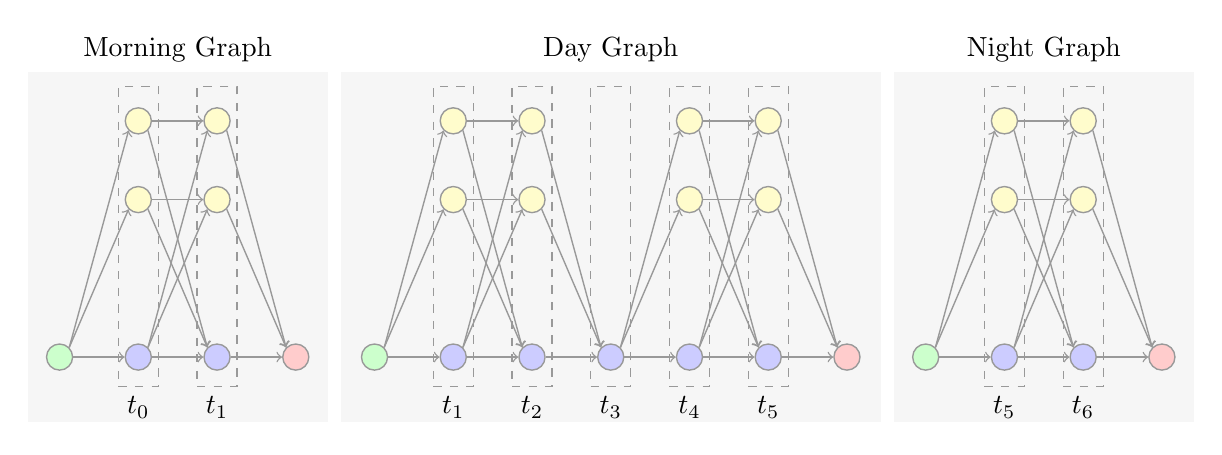
\begin{tikzpicture} 
		% morning graph
		\node[rectangle, fill=gray!7, minimum width=1.5in, minimum height=1.75in, label=above:Morning Graph](mBox) at (-2.5,1.4){};
		\node[rectangle, draw=black!40, dashed, minimum width=0.2in, minimum height = 1.5in, label=below:$t_0$](boxT0) at (-3,1.53){};
		\node[rectangle, draw=black!40, dashed, minimum width=0.2in, minimum height = 1.5in, label=below:$t_1$](boxT0) at (-2,1.53){};
		\node[circle, fill=green!20, line width=0.5pt, draw=black!40, minimum size=0.1in](mOne) at (-4,0){};
		\node[circle, fill=blue!20, line width=0.5pt, draw=black!40, minimum size=0.1in](mTwo) at (-3,0){}; 
		\node[circle, fill=blue!20, line width=0.5pt, draw=black!40, minimum size=0.1in](mThree) at (-2,0){};
		\node[circle, fill=red!20, line width=0.5pt, draw=black!40, minimum size=0.1in](mFour) at (-1,0){};

		\node[circle, fill=yellow!20, line width=0.5pt, draw=black!40, minimum size=0.1in](mFive) at (-3,2){};
		\node[circle, fill=yellow!20, line width=0.5pt, draw=black!40, minimum size=0.1in](mSix) at (-2,2){};
		\node[circle, fill=yellow!20, line width=0.5pt, draw=black!40, minimum size=0.1in](mSeven) at (-3,3){};
		\node[circle, fill=yellow!20, line width=0.5pt, draw=black!40, minimum size=0.1in](mEight) at (-2,3){};

		\draw[->, line width=0.5pt, color=black!40] (mOne.east) -- (mTwo.west){};
		\draw[->, line width=0.5pt, color=black!40] (mTwo.east) -- (mThree.west){};
		\draw[->, line width=0.5pt, color=black!40] (mThree.east) -- (mFour.west){};

		\draw[->, line width=0.5pt, color=black!40] (mOne.north east) -- (mFive.south west){};
		\draw[->, line width=0.5pt, color=black!40] (mTwo.north east) -- (mSix.south west){};
		\draw[->, line width=0.5pt, color=black!40] (mOne.north east) -- (mSeven.south west){};
                \draw[->, line width=0.5pt, color=black!40] (mTwo.north east) -- (mEight.south west){};

                \draw[->, line width=0.5pt, color=black!40] (mFive.south east) -- (mThree.north west){}; 
                \draw[->, line width=0.5pt, color=black!40] (mSix.south east) -- (mFour.north west){};
                \draw[->, line width=0.5pt, color=black!40] (mSeven.south east) -- (mThree.north west){};
		\draw[->, line width=0.5pt, color=black!40] (mEight.south east) -- (mFour.north west){};

                \draw[->, line width=0.5pt, color=black!40] (mFive.east) -- (mSix.west){};
                \draw[->, line width=0.5pt, color=black!40] (mSeven.east) -- (mEight.west){};

		% night graph
		\node[rectangle, fill=gray!7, minimum width=1.5in, minimum height=1.75in, label=above:Night Graph](nBox) at (8.5,1.4){};
		\node[rectangle, draw=black!40, dashed, minimum width=0.2in, minimum height = 1.5in, label=below:$t_6$](boxT2) at (9,1.53){};
		\node[rectangle, draw=black!40, dashed, minimum width=0.2in, minimum height = 1.5in, label=below:$t_5$](boxT0) at (8,1.53){};
		\node[circle, fill=green!20, line width=0.5pt, draw=black!40, minimum size=0.1in](nOne) at (7,0){};
		\node[circle, fill=blue!20, line width=0.5pt, draw=black!40, minimum size=0.1in](nTwo) at (8,0){}; 
		\node[circle, fill=blue!20, line width=0.5pt, draw=black!40, minimum size=0.1in](nThree) at (9,0){};
		\node[circle, fill=red!20, line width=0.5pt, draw=black!40, minimum size=0.1in](nFour) at (10,0){};

		\node[circle, fill=yellow!20, line width=0.5pt, draw=black!40, minimum size=0.1in](nFive) at (8,2){};
		\node[circle, fill=yellow!20, line width=0.5pt, draw=black!40, minimum size=0.1in](nSix) at (9,2){};
		\node[circle, fill=yellow!20, line width=0.5pt, draw=black!40, minimum size=0.1in](nSeven) at (8,3){};
		\node[circle, fill=yellow!20, line width=0.5pt, draw=black!40, minimum size=0.1in](nEight) at (9,3){};

		\draw[->, line width=0.5pt, color=black!40] (nOne.east) -- (nTwo.west){};
		\draw[->, line width=0.5pt, color=black!40] (nTwo.east) -- (nThree.west){};
		\draw[->, line width=0.5pt, color=black!40] (nThree.east) -- (nFour.west){};

		\draw[->, line width=0.5pt, color=black!40] (nOne.north east) -- (nFive.south west){};
		\draw[->, line width=0.5pt, color=black!40] (nTwo.north east) -- (nSix.south west){};
		\draw[->, line width=0.5pt, color=black!40] (nOne.north east) -- (nSeven.south west){};
                \draw[->, line width=0.5pt, color=black!40] (nTwo.north east) -- (nEight.south west){};

                \draw[->, line width=0.5pt, color=black!40] (nFive.south east) -- (nThree.north west){}; 
                \draw[->, line width=0.5pt, color=black!40] (nSix.south east) -- (nFour.north west){};
		\draw[->, line width=0.5pt, color=black!40] (nSeven.south east) -- (nThree.north west){};
		\draw[->, line width=0.5pt, color=black!40] (nEight.south east) -- (nFour.north west){};

		\draw[->, line width=0.5pt, color=black!40] (nFive.east) -- (nSix.west){};
                \draw[->, line width=0.5pt, color=black!40] (nSeven.east) -- (nEight.west){};


		% day graph	
		\node[rectangle, fill=gray!7, minimum width=2.7in, minimum height=1.75in, label=above:Day Graph](dBox) at (3,1.4){}; 
		\node[rectangle, draw=black!40, dashed, minimum width=0.2in, minimum height = 1.5in, label=below:$t_1$](boxT2) at (1,1.53){};
		\node[rectangle, draw=black!40, dashed, minimum width=0.2in, minimum height = 1.5in, label=below:$t_2$](boxT2) at (2,1.53){};
		\node[rectangle, draw=black!40, dashed, minimum width=0.2in, minimum height = 1.5in, label=below:$t_3$](boxT0) at (3,1.53){};
		\node[rectangle, draw=black!40, dashed, minimum width=0.2in, minimum height = 1.5in, label=below:$t_4$](boxT0) at (4,1.53){};
		\node[rectangle, draw=black!40, dashed, minimum width=0.2in, minimum height = 1.5in, label=below:$t_5$](boxT0) at (5,1.53){};
		\node[circle, fill=green!20, line width=0.5pt, draw=black!40, minimum size=0.1in](one) at (0,0){};
		\node[circle, fill=blue!20, line width=0.5pt, draw=black!40, minimum size=0.1in](two) at (1,0){}; 
		\node[circle, fill=blue!20, line width=0.5pt, draw=black!40, minimum size=0.1in](three) at (2,0){};
		\node[circle, fill=blue!20, line width=0.5pt, draw=black!40, minimum size=0.1in](four) at (3,0){};
		\node[circle, fill=blue!20, line width=0.5pt, draw=black!40, minimum size=0.1in](five) at (4,0){};
		\node[circle, fill=blue!20, line width=0.5pt, draw=black!40, minimum size=0.1in](six) at (5,0){};
		\node[circle, fill=red!20, line width=0.5pt, draw=black!40, minimum size=0.1in](seven) at (6,0){};
		
		\node[circle, fill=yellow!20, line width=0.5pt, draw=black!40, minimum size=0.1in](eight) at (1,2){};
		\node[circle, fill=yellow!20, line width=0.5pt, draw=black!40, minimum size=0.1in](nine) at (2,2){};
		\node[circle, fill=yellow!20, line width=0.5pt, draw=black!40, minimum size=0.1in](ten) at (4,2){};
		\node[circle, fill=yellow!20, line width=0.5pt, draw=black!40, minimum size=0.1in](eleven) at (5,2){};

		\node[circle, fill=yellow!20, line width=0.5pt, draw=black!40, minimum size=0.1in](twelve) at (1,3){};
		\node[circle, fill=yellow!20, line width=0.5pt, draw=black!40, minimum size=0.1in](thirteen) at (2,3){};
		\node[circle, fill=yellow!20, line width=0.5pt, draw=black!40, minimum size=0.1in](fourteen) at (4,3){};
		\node[circle, fill=yellow!20, line width=0.5pt, draw=black!40, minimum size=0.1in](fifteen) at (5,3){};

		\draw [->, line width=0.5pt, color=black!40] (one.east) -- (two.west);
		\draw [->, line width=0.5pt, color=black!40] (two.east) -- (three.west);
		\draw [->, line width=0.5pt, color=black!40] (three.east) -- (four.west);
		\draw [->, line width=0.5pt, color=black!40] (four.east) -- (five.west);
		\draw [->, line width=0.5pt, color=black!40] (five.east) -- (six.west);
		\draw [->, line width=0.5pt, color=black!40] (six.east) -- (seven.west);

		\draw [->, line width=0.5pt, color=black!40] (one.north east) -- (eight.south west);
		\draw [->, line width=0.5pt, color=black!40] (two.north east) -- (nine.south west);
		\draw [->, line width=0.5pt, color=black!40] (four.north east) -- (ten.south west);
		\draw [->, line width=0.5pt, color=black!40] (five.north east) -- (eleven.south west);
		\draw [->, line width=0.5pt, color=black!40] (eight.south east) -- (three.north west);
		\draw [->, line width=0.5pt, color=black!40] (nine.south east) -- (four.north west);
		\draw [->, line width=0.5pt, color=black!40] (ten.south east) -- (six.north west);
		\draw [->, line width=0.5pt, color=black!40] (eleven.south east) -- (seven.north west);
		\draw [->, line width=0.5pt, color=black!40] (eight.east) -- (nine.west);
		\draw [->, line width=0.5pt, color=black!40] (ten.east) -- (eleven.west); 

		\draw [->, line width=0.5pt, color=black!40] (one.north east) -- (twelve.south west);
		\draw [->, line width=0.5pt, color=black!40] (two.north east) -- (thirteen.south west);
		\draw [->, line width=0.5pt, color=black!40] (four.north east) -- (fourteen.south west);
		\draw [->, line width=0.5pt, color=black!40] (five.north east) -- (fifteen.south west);
		\draw [->, line width=0.5pt, color=black!40] (twelve.south east) -- (three.north west);
		\draw [->, line width=0.5pt, color=black!40] (thirteen.south east) -- (four.north west);
		\draw [->, line width=0.5pt, color=black!40] (fourteen.south east) -- (six.north west);
		\draw [->, line width=0.5pt, color=black!40] (fifteen.south east) -- (seven.north west);
		\draw [->, line width=0.5pt, color=black!40] (twelve.east) -- (thirteen.west);
		\draw [->, line width=0.5pt, color=black!40] (fourteen.east) -- (fifteen.west); 
	\end{tikzpicture}
	\caption{Night and day graphs.}
	\label{fig:nightVsDayGraph}
\end{figure*}


\begin{figure*}
	\centering
	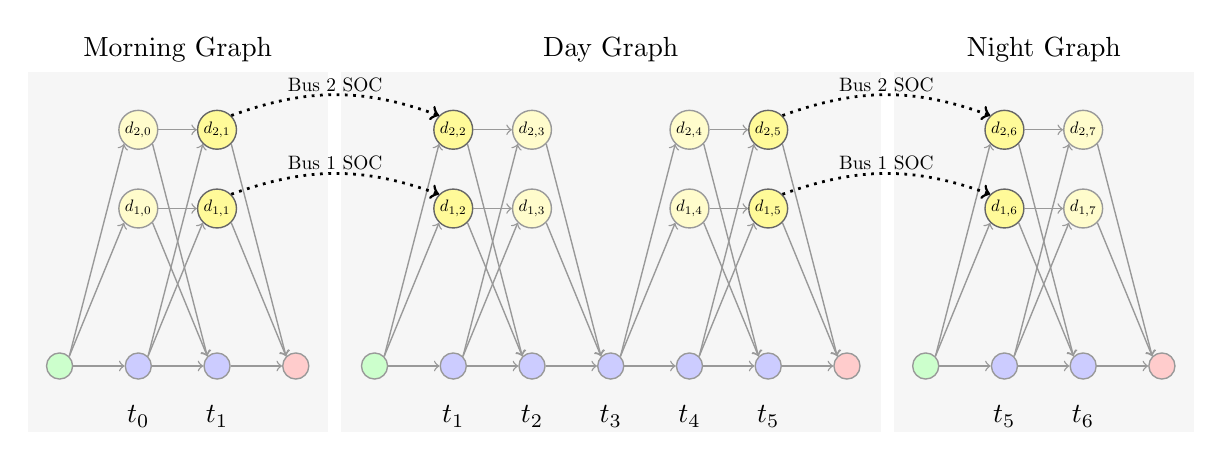
\begin{tikzpicture} 
		% morning graph
		\node[rectangle, fill=gray!7, minimum width=1.5in, minimum height=1.8in, label=above:Morning Graph](mBox) at (-2.5,1.45){};
		\node[rectangle, minimum width=0.2in, minimum height = 1.5in, label=below:$t_0$](boxT0) at (-3,1.53){};
		\node[rectangle, minimum width=0.2in, minimum height = 1.5in, label=below:$t_1$](boxT0) at (-2,1.53){};
		\node[circle, fill=green!20, line width=0.5pt, draw=black!40, minimum size=0.1in](mOne) at (-4,0){};
		\node[circle, fill=blue!20, line width=0.5pt, draw=black!40, minimum size=0.1in](mTwo) at (-3,0){};
		\node[circle, fill=blue!20, line width=0.5pt, draw=black!40, minimum size=0.1in](mThree) at (-2,0){};
		\node[circle, fill=red!20, line width=0.5pt, draw=black!40, minimum size=0.1in](mFour) at (-1,0){};

		\node[circle, fill=yellow!20, line width=0.5pt, draw=black!40, minimum size=0.1in, inner sep=1pt](mFive) at (-3,2){\scalebox{0.6}{$d_{1,0}$}};
		\node[circle, fill=yellow!40, line width=0.5pt, draw=black!60, minimum size=0.1in, inner sep=1pt](mSix) at (-2,2){\scalebox{0.6}{$d_{1,1}$}};
		\node[circle, fill=yellow!20, line width=0.5pt, draw=black!40, minimum size=0.1in, inner sep=1pt](mSeven) at (-3,3){\scalebox{0.6}{$d_{2,0}$}};
		\node[circle, fill=yellow!40, line width=0.5pt, draw=black!60, minimum size=0.1in, inner sep=1pt](mEight) at (-2,3){\scalebox{0.6}{$d_{2,1}$}};

		\draw[->, line width=0.5pt, color=black!40] (mOne.east) -- (mTwo.west){};
		\draw[->, line width=0.5pt, color=black!40] (mTwo.east) -- (mThree.west){};
		\draw[->, line width=0.5pt, color=black!40] (mThree.east) -- (mFour.west){};

		\draw[->, line width=0.5pt, color=black!40] (mOne.north east) -- (mFive.south west){};
		\draw[->, line width=0.5pt, color=black!40] (mTwo.north east) -- (mSix.south west){};
		\draw[->, line width=0.5pt, color=black!40] (mOne.north east) -- (mSeven.south west){};
                \draw[->, line width=0.5pt, color=black!40] (mTwo.north east) -- (mEight.south west){};

                \draw[->, line width=0.5pt, color=black!40] (mFive.south east) -- (mThree.north west){}; 
                \draw[->, line width=0.5pt, color=black!40] (mSix.south east) -- (mFour.north west){};
                \draw[->, line width=0.5pt, color=black!40] (mSeven.south east) -- (mThree.north west){};
		\draw[->, line width=0.5pt, color=black!40] (mEight.south east) -- (mFour.north west){};

                \draw[->, line width=0.5pt, color=black!40] (mFive.east) -- (mSix.west){};
                \draw[->, line width=0.5pt, color=black!40] (mSeven.east) -- (mEight.west){};

		% night graph
		\node[rectangle, fill=gray!7, minimum width=1.5in, minimum height=1.8in, label=above:Night Graph](nBox) at (8.5,1.45){};
		\node[rectangle, minimum width=0.2in, minimum height = 1.5in, label=below:$t_6$](boxT2) at (9,1.53){};
		\node[rectangle, minimum width=0.2in, minimum height = 1.5in, label=below:$t_5$](boxT0) at (8,1.53){};
		\node[circle, fill=green!20, line width=0.5pt, draw=black!40, minimum size=0.1in](nOne) at (7,0){};
		\node[circle, fill=blue!20, line width=0.5pt, draw=black!40, minimum size=0.1in](nTwo) at (8,0){}; 
		\node[circle, fill=blue!20, line width=0.5pt, draw=black!40, minimum size=0.1in](nThree) at (9,0){};
		\node[circle, fill=red!20, line width=0.5pt, draw=black!40, minimum size=0.1in](nFour) at (10,0){};

		\node[circle, fill=yellow!40, line width=0.5pt, draw=black!60, minimum size=0.1in, inner sep=1pt](nFive) at (8,2){\scalebox{0.6}{$d_{1,6}$}};
		\node[circle, fill=yellow!20, line width=0.5pt, draw=black!40, minimum size=0.1in, inner sep=1pt](nSix) at (9,2){\scalebox{0.6}{$d_{1,7}$}};
		\node[circle, fill=yellow!40, line width=0.5pt, draw=black!60, minimum size=0.1in, inner sep=1pt](nSeven) at (8,3){\scalebox{0.6}{$d_{2,6}$}};
		\node[circle, fill=yellow!20, line width=0.5pt, draw=black!40, minimum size=0.1in, inner sep=1pt](nEight) at (9,3){\scalebox{0.6}{$d_{2,7}$}};

		\draw[->, line width=0.5pt, color=black!40] (nOne.east) -- (nTwo.west){};
		\draw[->, line width=0.5pt, color=black!40] (nTwo.east) -- (nThree.west){};
		\draw[->, line width=0.5pt, color=black!40] (nThree.east) -- (nFour.west){};

		\draw[->, line width=0.5pt, color=black!40] (nOne.north east) -- (nFive.south west){};
		\draw[->, line width=0.5pt, color=black!40] (nTwo.north east) -- (nSix.south west){};
		\draw[->, line width=0.5pt, color=black!40] (nOne.north east) -- (nSeven.south west){};
                \draw[->, line width=0.5pt, color=black!40] (nTwo.north east) -- (nEight.south west){};

                \draw[->, line width=0.5pt, color=black!40] (nFive.south east) -- (nThree.north west){}; 
                \draw[->, line width=0.5pt, color=black!40] (nSix.south east) -- (nFour.north west){};
		\draw[->, line width=0.5pt, color=black!40] (nSeven.south east) -- (nThree.north west){};
		\draw[->, line width=0.5pt, color=black!40] (nEight.south east) -- (nFour.north west){};

		\draw[->, line width=0.5pt, color=black!40] (nFive.east) -- (nSix.west){};
                \draw[->, line width=0.5pt, color=black!40] (nSeven.east) -- (nEight.west){};


		% day graph	
		\node[rectangle, fill=gray!7, minimum width=2.7in, minimum height=1.8in, label=above:Day Graph](dBox) at (3,1.45){}; 
		\node[rectangle, minimum width=0.2in, minimum height = 1.5in, label=below:$t_1$](boxT2) at (1,1.53){};
		\node[rectangle, minimum width=0.2in, minimum height = 1.5in, label=below:$t_2$](boxT2) at (2,1.53){};
		\node[rectangle, minimum width=0.2in, minimum height = 1.5in, label=below:$t_3$](boxT0) at (3,1.53){};
		\node[rectangle, minimum width=0.2in, minimum height = 1.5in, label=below:$t_4$](boxT0) at (4,1.53){};
		\node[rectangle, minimum width=0.2in, minimum height = 1.5in, label=below:$t_5$](boxT0) at (5,1.53){};
		\node[circle, fill=green!20, line width=0.5pt, draw=black!40, minimum size=0.1in](one) at (0,0){};
		\node[circle, fill=blue!20, line width=0.5pt, draw=black!40, minimum size=0.1in](two) at (1,0){}; 
		\node[circle, fill=blue!20, line width=0.5pt, draw=black!40, minimum size=0.1in](three) at (2,0){};
		\node[circle, fill=blue!20, line width=0.5pt, draw=black!40, minimum size=0.1in](four) at (3,0){};
		\node[circle, fill=blue!20, line width=0.5pt, draw=black!40, minimum size=0.1in](five) at (4,0){};
		\node[circle, fill=blue!20, line width=0.5pt, draw=black!40, minimum size=0.1in](six) at (5,0){};
		\node[circle, fill=red!20, line width=0.5pt, draw=black!40, minimum size=0.1in](seven) at (6,0){};
		
		\node[circle, fill=yellow!40, line width=0.5pt, draw=black!60, minimum size=0.1in, inner sep=1pt](eight) at (1,2){\scalebox{0.6}{$d_{1,2}$}};
		\node[circle, fill=yellow!20, line width=0.5pt, draw=black!40, minimum size=0.1in, inner sep=1pt](nine) at (2,2){\scalebox{0.6}{$d_{1,3}$}};
		\node[circle, fill=yellow!20, line width=0.5pt, draw=black!40, minimum size=0.1in, inner sep=1pt](ten) at (4,2){\scalebox{0.6}{$d_{1,4}$}};
		\node[circle, fill=yellow!40, line width=0.5pt, draw=black!60, minimum size=0.1in, inner sep=1pt](eleven) at (5,2){\scalebox{0.6}{$d_{1,5}$}};

		\node[circle, fill=yellow!40, line width=0.5pt, draw=black!60, minimum size=0.1in, inner sep=1pt](twelve) at (1,3){\scalebox{0.6}{$d_{2,2}$}};
		\node[circle, fill=yellow!20, line width=0.5pt, draw=black!40, minimum size=0.1in, inner sep=1pt](thirteen) at (2,3){\scalebox{0.6}{$d_{2,3}$}};
		\node[circle, fill=yellow!20, line width=0.5pt, draw=black!40, minimum size=0.1in, inner sep=1pt](fourteen) at (4,3){\scalebox{0.6}{$d_{2,4}$}};
		\node[circle, fill=yellow!40, line width=0.5pt, draw=black!60, minimum size=0.1in, inner sep=1pt](fifteen) at (5,3){\scalebox{0.6}{$d_{2,5}$}};

		\draw [->, line width=0.5pt, color=black!40] (one.east) -- (two.west);
		\draw [->, line width=0.5pt, color=black!40] (two.east) -- (three.west);
		\draw [->, line width=0.5pt, color=black!40] (three.east) -- (four.west);
		\draw [->, line width=0.5pt, color=black!40] (four.east) -- (five.west);
		\draw [->, line width=0.5pt, color=black!40] (five.east) -- (six.west);
		\draw [->, line width=0.5pt, color=black!40] (six.east) -- (seven.west);

		\draw [->, line width=0.5pt, color=black!40] (one.north east) -- (eight.south west);
		\draw [->, line width=0.5pt, color=black!40] (two.north east) -- (nine.south west);
		\draw [->, line width=0.5pt, color=black!40] (four.north east) -- (ten.south west);
		\draw [->, line width=0.5pt, color=black!40] (five.north east) -- (eleven.south west);
		\draw [->, line width=0.5pt, color=black!40] (eight.south east) -- (three.north west);
		\draw [->, line width=0.5pt, color=black!40] (nine.south east) -- (four.north west);
		\draw [->, line width=0.5pt, color=black!40] (ten.south east) -- (six.north west);
		\draw [->, line width=0.5pt, color=black!40] (eleven.south east) -- (seven.north west);
		\draw [->, line width=0.5pt, color=black!40] (eight.east) -- (nine.west);
		\draw [->, line width=0.5pt, color=black!40] (ten.east) -- (eleven.west); 

		\draw [->, line width=0.5pt, color=black!40] (one.north east) -- (twelve.south west);
		\draw [->, line width=0.5pt, color=black!40] (two.north east) -- (thirteen.south west);
		\draw [->, line width=0.5pt, color=black!40] (four.north east) -- (fourteen.south west);
		\draw [->, line width=0.5pt, color=black!40] (five.north east) -- (fifteen.south west);
		\draw [->, line width=0.5pt, color=black!40] (twelve.south east) -- (three.north west);
		\draw [->, line width=0.5pt, color=black!40] (thirteen.south east) -- (four.north west);
		\draw [->, line width=0.5pt, color=black!40] (fourteen.south east) -- (six.north west);
		\draw [->, line width=0.5pt, color=black!40] (fifteen.south east) -- (seven.north west);
		\draw [->, line width=0.5pt, color=black!40] (twelve.east) -- (thirteen.west);
		\draw [->, line width=0.5pt, color=black!40] (fourteen.east) -- (fifteen.west); 


		\draw [dotted, color=black,-,line width=1pt] (mSix.north east) edge[->,bend left=20pt]node[above=-2.5pt]{\scalebox{0.7}{Bus 1 SOC}}(eight.north west); 
		\draw [dotted, color=black,-,line width=1pt] (mEight.north east) edge[->,bend left=20pt]node[above=-2.5pt]{\scalebox{0.7}{Bus 2 SOC}}(twelve.north west);

		\draw [dotted, color=black,-,line width=1pt] (eleven.north east) edge[->,bend left=20pt]node[above=-2.5pt]{\scalebox{0.7}{Bus 1 SOC}}(nFive.north west); 
		\draw [dotted, color=black,-,line width=1pt] (fifteen.north east) edge[->,bend left=20pt]node[above=-2.5pt]{\scalebox{0.7}{Bus 2 SOC}}(nSeven.north west);
	\end{tikzpicture}
	\caption{Bus SOC between night and day graphs.}
	\label{fig:nightVsDayConnected}
\end{figure*}

\section{Objective Function}
The objective function in this work models the rate schedule used in \cite{noauthor_rocky_nodate}, where the result is modeled as the monthly charge a transit authority might receive from the power provider. The objective function includes charges for energy, power, and facility use and implements both on and off-peak rates.
\subsection{Energy}
\par Energy charges are given per Kilowatt-hour of energy consumed and include power from external loads and bus chargers. Let $\mathbf{p}$ be the average external power used at each timestep, where $\mathbf{p}_i$ is the average power draw between $t_j$ and $t_{j + 1}$. The energy consumed by external loads from $t_j$ to $t_{j+1}$ is computed as 
\begin{equation}
	e_{l_j} = \mathbf{p}_i \times \Delta_t,
\end{equation}
where $\Delta_t$ is the change in time from $t_j$ to $t_{j+1}$ in hours. The energy consumed by bus chargers for the same interval is computed as  
\begin{equation}
	e_{b_j} = \sum_{k\in t}g_{i,k,l},	
\end{equation}
which sums all changes in bus SOC between $t_j$ and $t_{j+1}$.
The total energy is computed as 
\begin{equation}\label{eqn:energy1}
	e_j = e_{l_j} + e_{b_j}
\end{equation}
The equation for \ref{eqn:energy1} can be written in standard form as 
\begin{equation}\label{eqn:energy2}
	\begin{aligned}
		e_j -\sum_{k\in t}g_{i,k,l} &= p_i \times \Delta_t \\
		\begin{bmatrix} 1_{e_j} & -1_{g_1} & \hdots -1_{g_n} \end{bmatrix} \begin{bmatrix}e_j \\ g_1 \\ \vdots \\ g_n \end{bmatrix} &= p_i \times \Delta_t
	\end{aligned}
\end{equation}
Equation \ref{eqn:energy2} can be modified to reflect the energy consumed in an arbitrary time period, $T$, by including the corresponding values for $g$ and $p$ as
\begin{equation}\label{eqn:energy3}
	\begin{aligned}
	e_j -\sum_{k\in T}g_{i,k,l} &= \left ( \sum_{i\in T}p_i \right ) \times \Delta_t \\
		\begin{bmatrix} 1_{e_j} & -1_{g_1} & \hdots -1_{g_n} \end{bmatrix} \begin{bmatrix}e_j \\ g_1 \\ \vdots \\ g_n \end{bmatrix} &= e_{p_j}.
	\end{aligned}
\end{equation}
For multiple time periods, the constraint can be expanded in matrix form, where row $i$ corresponds to the periods of time in $T_i$. Furthermore, by including $e_j$ in the solution vector $\mathbf{y}$ and zero-padding appropriately, the expanded form of equation \ref{eqn:energy3} can be written as  
\begin{equation}
	E\mathbf{y} = \mathbf{e}_p,
\end{equation}
where row $i$ in $E$ reflects equation \ref{eqn:energy3} for the time intervals in $T_i$, and $\mathbf{e}_{p_i}$ contains the energy from external loads during $T_i$.
The day is divided into on and off-peak times.  on-peak times reflect periods where high power use is common.
\subsection{Power}
Power charges are computed for the maximum average power draw, where the average is computed over a 15 minute sliding window. The average power can be computed as the energy in the window divided by the window length in hours. In this case, a 15 minute window equates to a quarter hour. Let $\bar{p}_j$ be the average power from $j - 15$ to $j$. Equation \ref{eqn:energy3} can be adapted to compute the average power as
\begin{equation}\label{eqn:power1} 
	\begin{aligned}
		\bar{p}_j - \left ( \sum_{k\in T_j}g_{i,k,l} \right )/4 &= \left ( \sum_{i\in T_j}p_i \right ) \times \frac{\Delta_t}{4} \\
		\begin{bmatrix} 1_{\bar{p}_j} & -\frac{1_{g_1}}{4} & \hdots -\frac{1_{g_n}}{4} \end{bmatrix} \begin{bmatrix}e_j \\ g_1 \\ \vdots \\ g_n \end{bmatrix} &= \frac{p_T \times \Delta_t}{4}.
	\end{aligned}
\end{equation}
Equation \ref{eqn:power1} can further be expanded and zero padded to compute the average power at each time, $t_i$ by applying equation \ref{eqn:power1} to the corresponding window as
\begin{equation}\label{eqn:power2}
	P\mathbf{y} = \mathbf{p}.	
\end{equation}
The maximum average power, denoted $\hat{p}$, is greater than or equal to each average power computed in equation \ref{eqn:power2}.  This yields an additional set of inequality constraints 
\begin{equation}\label{eqn:cPower1}
	\begin{aligned}
		 \begin{bmatrix} 
			-1_{\hat{p}} & 1_{\bar{p}_0} & 0             & \hdots & 0 \\ 
	        	-1_{\hat{p}} & 0       & 1_{\bar{p}_1} & \hdots & 0\\
			-1_{\hat{p}} & 0       & 0 & \hdots    & 1_{\bar{p}_j} \\
		 \end{bmatrix}\mathbf{y} &\le \mathbf{0} \\ 
		 P_{\text{max}}\mathbf{y} &\le \mathbf{0}.
	\end{aligned}
\end{equation}
Because the max average power is minimizied in the objective function, the value for $\hat{p}_{\text{max}}$ will be forced down to the value of the greatest average power computed in equation \ref{eqn:power2}, and accurately reflect the maximum average power.
\subsection{On/Off Peak Rates}
Power providers also divide each day into on and off-peak periods during which different rates are applied for both energy and power charges. Let $H$ and $L$ be the respective sets of all time indices in on and off peak periods. The cost of energy during on-peak hours can be expressed as 
\begin{equation}\label{eqn:cEnergy1}
	\begin{aligned}
		c_{\text{energy}_H} &= \left ( \sum_{j\in H} e_j \right ) r_{e_\text{on}} \\
		&= \begin{bmatrix}r_{e_1} & 0 & \hdots & 0 & r_{e_4} & \hdots & 0 \end{bmatrix}\mathbf{y} \\
		&= \mathbf{r}_{e_\text{on}}^T\mathbf{y},
	\end{aligned}
\end{equation}
where $\mathbf{r}_{e_\text{on}}$ contains the value of $r_{e_\text{on}}$ at the index corresponding to $e_j$ in $\mathbf{y} \ \forall j \in H$. A similar formulation can be used to describe the cost of energy consumed during off-peak hours.  
\par An on-peak rate also applies to charges for power. Equation \ref{eqn:cPower1} can be adapted to only include rows that correspond to average power values during on-peak hours such that
\begin{equation}\label{eqn:cPOnPeak} 
	\begin{aligned}
		 \begin{bmatrix} 
			 -1_{\hat{p}_\text{on}} & 1_{\bar{p}_0} & 0             & \hdots & 0 \\ 
			 -1_{\hat{p}_\text{on}} & 0       & 1_{\bar{p}_1} & \hdots & 0\\
			 -1_{\hat{p}_\text{on}} & 0       & 0 & \hdots    & 1_{\bar{p}_j} \\
		 \end{bmatrix}\mathbf{y} &\le \mathbf{0} \\ 
		 P_{\text{on}}\mathbf{y} &\le \mathbf{0}.  
	\end{aligned}
\end{equation}
Similarly, the off-peak max average power can be computed as  
\begin{equation}\label{eqn:cPOffPeak}
	\begin{aligned}
		 \begin{bmatrix} 
			 -1_{\hat{p}_\text{off}} & 1_{\bar{p}_0} & 0             & \hdots & 0 \\ 
			 -1_{\hat{p}_\text{off}} & 0       & 1_{\bar{p}_1} & \hdots & 0\\
			 -1_{\hat{p}_\text{off}} & 0       & 0 & \hdots    & 1_{\bar{p}_j} \\
		 \end{bmatrix}\mathbf{y} &\le \mathbf{0} \\ 
		 P_{\text{off}}\mathbf{y} &\le \mathbf{0},  
	\end{aligned}
\end{equation}
where each row corresponds to $\bar{p}_j \ \forall j \in L$.
\par Many power providers also include a facilities charge.  The facilities charge is billed for each Kw of the maximum average power in \textit{both} on and off-peak intervals. The total max average power is calculated using equation \ref{eqn:cPower1}.
\par The total power charge can be computed as the sum of the on-peak, off-peak, and facilities charges as 
\begin{equation}
	\begin{aligned}
		c_\text{power} &= \begin{bmatrix}r_{\hat{p}_{\text{on}}} & \hdots & 0 & r_{\hat{p}_{\text{off}}} & \hdots & r_{\hat{p}_{\text{facilities}}} \end{bmatrix}\mathbf{y} \\
			&= \mathbf{r}_{\hat{p}}^T\mathbf{y}
	\end{aligned}
\end{equation}

\subsection{Objective Function}
The objective function combines the cost of energy and power, where the on-peak and off-peak energy is combined as 
\begin{equation}\label{eqn:cEnergy2}
	\begin{aligned}
		c_{\text{energy}} &= \mathbf{r}_{e_\text{on}}^T\mathbf{y} + \mathbf{r}_{e_\text{off}}^T\mathbf{y} \\
		&=\left ( \mathbf{r}_{e_\text{on}} + \mathbf{r}_{e_\text{off}} \right )^T \mathbf{y} \\
		&= \mathbf{r}_e^T\mathbf{y}.
	\end{aligned}
\end{equation}
The combined expression is given as 
\begin{equation}\label{eqn:objective}
	\begin{aligned}
		c_{\text{total}} &= c_{\text{power}} + c_{\text{energy}} \\ 
				 &= \mathbf{r}_e^T\mathbf{y} + \mathbf{r}_{\hat{p}}^T\mathbf{y} \\
				 &= \left ( \mathbf{r}_e + \mathbf{r}_{\hat{p}} \right )^T\mathbf{y} \\
				 &= \mathbf{r}^T\mathbf{y}.
	\end{aligned}
\end{equation}
\par Equation \ref{eqn:objective} is used as the objective function in a mixed integer linear program of the form
\begin{equation}
	\begin{aligned}
		& \underset{\mathbf{y}}{\scalebox{1}{\text{min}}} \ \mathbf{r}^T\mathbf{y} \\
		\text{subject to}& \ \ \ \  C_{\text{eq}}\mathbf{y} = \mathbf{c}_{\text{eq}}, \ C_{\text{ineq}}\mathbf{y} \le \mathbf{c}_{\text{ineq}},
	\end{aligned}
\end{equation}
Where $C_{\text{eq}}, \mathbf{c}_{\text{eq}}, C_{\text{ineq}}, and \mathbf{c}_{text{ineq}}$ are formed by stacking the equality and inequality constraints from equations \ref{eqn:flow}, \ref{eqn:cGroupFlow}, \ref{eqn:cSocFinal}, \ref{eqn:power2}, \ref{eqn:cPower1}, \ref{eqn:cPOnPeak}, and \ref{eqn:cPOffPeak}.
\begin{equation}
	\begin{aligned}
		& \underset{\mathbf{y}}{\scalebox{1}{\text{min}}} \ \mathbf{r}^T\mathbf{y} \\
		\text{subject to}& \ \ \ \  \begin{bmatrix}
			\begin{bmatrix}A & 0 \end{bmatrix} \\
				D_{\text{eq}} \\
				P
				\end{bmatrix} \mathbf{y} = \begin{bmatrix}c_f \\ \mathbf{d}_{\text{eq}}\\\mathbf{p} \end{bmatrix}, \ \begin{bmatrix}
		\begin{bmatrix} B & 0 \end{bmatrix} \\
			D_{\text{ineq}} \\ 
			P_{\text{max}} \\
			P_{\text{on}} \\
			P_{\text{off}}
			\end{bmatrix}\mathbf{y} \le \begin{bmatrix}\mathbf{1} \\ \mathbf{d}_{\text{ineq}} \\ \mathbf{0} \\ \mathbf{0} \\ \mathbf{0} \end{bmatrix},
	\end{aligned}
\end{equation}



\section{Results}
This section contains analysis and results of the planning framework and is subdivided into three subsections: uncontested results, contested results, and multi-rate comparisons.  
\subsection{Baseline and Setup}
The several experiments in this section compare the results of the the framework given in equation \ref{eqn:finalObjective} with a baseline. The baseline attempts to model the general behavior of a stereotypical bus driver. From conversations with the Utah Transit Authority (UTA), bus drivers generally enter the station and top off their bus's battery if a charger is available. The baseline reflects the bus driver behavior with an objetive function which maximizes the number of instances where a bus plugs in. The number of plug-in instances can be computed as the sum of group flow values and results in the objetive function
\begin{equation}
	\underset{\mathbf{y}}{\text{max}} \ \mathbf{1}^TB\mathbf{y},
\end{equation}
\par All other constraints are held equal, resulting in a baseline formulation given as
\begin{equation}\label{eqn:finalBaselineObjective}
	\begin{matrix*}[c]
		\underset{\mathbf{y}}{\scalebox{1}{\text{max}}} \ \mathbf{1}^TB\mathbf{y} \ \text{subject to}\\
		\begin{bmatrix*}[l]
				\tilde{A} \\
				D_{\text{eq}} \\
				P
				\end{bmatrix*} \mathbf{y} = \begin{bmatrix*}[l]\mathbf{c}_f \\ \mathbf{d}_{\text{eq}}\\\mathbf{p} \end{bmatrix*}, \ \begin{bmatrix*}[l]
			\tilde{B} \\
			D_{\text{ineq}} \\ 
			P_{\text{max}} \\
			P_{\text{on}} \\
			P_{\text{off}}
			\end{bmatrix*}\mathbf{y} \le \begin{bmatrix*}\mathbf{1} \\ \mathbf{d}_{\text{ineq}} \\ \mathbf{0} \\ \mathbf{0} \\ \mathbf{0} \end{bmatrix*}
	\end{matrix*}.
\end{equation}
	\par Additionally, each experiment is run in five minute increments such that $t_k$ represents a time instance five minutes behind $t_{k+1}$.  START HERE == was working to find how long for a full charge to justify a bar. will fill in bar charts with this value as well.

\subsection{Uncontested Results}
This section compares the charge schedule associated with equation \ref{eqn:finalObjective} with a schedule developed by a baseline algorithm.  The baseline adheres to all the constraints given previously, but maximizes the objective 
\begin{equation}
	\underset{\mathbf{y}}{\text{max}} \ \mathbf{1}^TB\mathbf{y},
\end{equation}
which incentivizes bus charging when possible. An initial cost comparison is given for an uncontested scenario where the number of chargers is equal to the number of buses. The cost breakdown is given in figure \ref{fig:costComparison}.
\begin{figure}
	\centering
	\makeComparisonBarChart{media/costComparison5Bus5Chargers.csv}{Cost (Dollars)}{Baseline}{Optimized}
	\caption{Cost Comparison between optimized and baseline algorithms}
	\label{fig:costComparison}
\end{figure}
\par Note how the energy charge is equivalent, which indicates that similar amounts of energy were consumed in both scenarios. Dispite the similarity in energy consumption, however, facilities and on-peak power chargers are significantly larger for the unoptimized schedule. 
\par Figure \ref{fig:totalPower1} compares the average power use between the optimized and baseline algorithms. There are two primary differences between the two. The first is that the optimized schedule avoids charging during on-peak hours.  The second is how the optimized charge schedule regulates each charge event to spread the power draw over larger, intermittent periods of time. Avoiding the on-peak time window and minimizing average power draw resulted in the cost disparities shown in figure \ref{fig:costComparison}.

\begin{figure*}
	\centering
	\makeComparisonTotalPower{media/baseline5Bus5ChargerTotalPowerPlot.csv}{media/optimized5Bus5ChargerTotalPowerPlot.csv}{15-Minute Average Power (kW)}{Baseline}{Optimized}
	\caption{15-Minute AVerage Power for one day}
	\label{fig:totalPower1}
\end{figure*} 
Figure \ref{fig:powerPlot1} separates the power draw into power from external loads and power used by buses and shows again how bus charging was optimized to avoid on-peak hours and spread power use over time.  
\begin{figure*}
	\centering
	\makeComparisonPower{media/baseline5Bus5ChargerPowerPlot.csv}{media/optimized5Bus5ChargerPowerPlot.csv}{15-Minute AVerage Power (kW)}{Baseline}{Optimized}
	\caption{Comparison between uncontrolled and bus loads}
	\label{fig:powerPlot1}
\end{figure*}

\subsection{Contested Results}
An optimized schedule can also be produced in resource contested environments. Contention occures when the number of chargers is scarce in comparison to the number of buses and can require that buses charge in disoptimal circumstances.  For example, if charging resources are saturated during off-peak hours, other buses might be forced to charge in the on-peak window. 
\par Figure \ref{fig:contention1} shows the monthly cost from a scenario with one charger and multiple buses. Note the minimial cost increase per bus.  Each subsequent bus incurs a minimal additional cost, showing that charge plans also minimize charge in the presence of contention.
\begin{figure}
	\begin{tikzpicture}
		\begin{axis}[SmallPointPlot, xlabel=Number of Buses, ylabel=Total Monthly Cost, ymin=3000, xmax=11]
			\addplot[blue, only marks, mark size=3pt] coordinates {(5,3034.35) (6,3108.23) (7,3174.54) (8,3255.87) (9,3313.43) (10, 3391.16) (11, 3463.42)}; 
			\addplot[blue] coordinates {(5,3034.35) (6,3108.23) (7,3174.54) (8,3255.87) (9,3313.43) (10, 3391.16) (11, 3463.42)};
		\end{axis}
	\end{tikzpicture}
	\caption{Results for several single charger scenarios.}
	\label{fig:contention1}
\end{figure}
\par Figure \ref{fig:contention2} demonstrates how cost is minimized in the presence of contention. Figure \ref{fig:contention2} compares loads between a 5 and 11 bus scenario, where only one charger is given and the uncontrolled loads are equivalent. In the 5 bus scenario, loads are distributed amongst off-peak hours, resulting in an optimized cost.  The 11 bus scenario requires significantly more power and is forced to charge during on-peak hours.  Note however that average power use is kept relatively low and seldom increases the maximum average power for on-peak use. Both scenarios also make ample use of night charging, where the number of chargers is the same as the number of buses.  
\begin{figure*}
	\centering
	\makeComparisonPower{media/optimized5Bus1ChargerPowerPlot.csv}{media/optimized11Bus1ChargerPowerPlot.csv}{15-Minute AVerage Power (kW)}{5 Bus Scenario}{11 Bus Scenario}
	\caption{Comparison of the loads for a 5 and 11 bus scenario with one overhead charger} 
	\label{fig:contention2}
\end{figure*}

\subsection{Multi-Rate Comparison}
Figure \ref{fig:multiRateCostComparison} shows the comparison between multi and single-rate charging. Both scenarios include 5 buses and 1 charger. As shown in figure \ref{fig:multiRateCostComparison}, the cost difference is marginal at best.  The cost of the multi-rate scenario is \$3006.94 and the cost of the single-rate scenario is \$3007.77. 
\begin{figure}
	\centering
	\makeComparisonBarChart{media/costComparisonMultiVsSingle.csv}{Cost (Dollars)}{Multi-Rate}{Single-Rate}
	\caption{Cost Comparison between a multi-rate and single-rate charge schedule}
	\label{fig:multiRateCostComparison}
\end{figure}
The small cost decrease is also consistent with larger scenarios as shown in figure \ref{fig:costComparisonMultiVsSingleLarge}. 
\par Upon further observation, maximum charge edges in multi-rate scenarios are used more frequently than their low-charge counterparts as shown in figure \ref{fig:chargeRateHistogram}. This would help explain the similarities in cost. If the highest rate is almost always selected, then the resulting plan would resemble a single-rate schedule.  
\begin{figure}
	\makeComparisonBarChart{media/costComparisonMultiVsSingleLarge.csv}{Cost (Dollars)}{Multi-Rate}{Single-Rate}
	\caption{Cost Comaprison between multi and single rate charging for a 35 bus 6 charger scenario}
	\label{fig:costComparisonMultiVsSingleLarge}
\end{figure}
\par Cost is also based on the average instantanous power. Because both single and multi-rate plans charge buses in relatively small time periods the average power use is kept relatively low (see figures \ref{fig:contention2}, and \ref{fig:contention1}). There are also many circumstances when a bus's charge time is limited, resulting in high charge rates.
\begin{figure}
	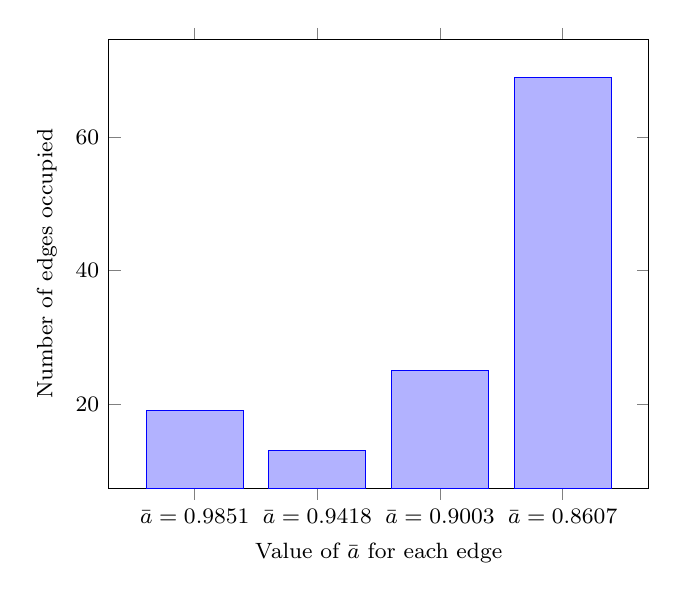
\begin{tikzpicture}
		\begin{axis}[ybar, xmin=0.3, xmax=4.7, font=\footnotesize, xtick={1,2,3,4},xticklabels={$\bar{a} = 0.9851$,$\bar{a} = 0.9418$,$\bar{a} = 0.9003$,$\bar{a} = 0.8607$},
			xlabel=Value of $\bar{a}$ for each edge, ylabel=Number of edges occupied, bar width=35pt]
			\addplot coordinates{(1,19) (2,13) (3,25) (4,69)};
		\end{axis}
	\end{tikzpicture}
	\caption{Histogram of charge rates}
	\label{fig:chargeRateHistogram}
\end{figure}














\section{Conclusions and Future Work }
In conclusion, the charge schedules developed in equation (\ref{eqn:finalObjective}) yield significant cost savings over both the baseline and the work by \cite{He_2022_Battery}. These savings come from minimizing the average power consumption, and charging during off-peak hours. Cost savings are maintained in both uncontested and resource constrained scenarios.  There is also little to be gained by offering multiple charge rates because average power can be managed with high charge rates by reducing the charge duration. Furthermore, it was shown that when given the choice, the optimizer primarily selected high charge rates, which reduces the problem complexity to the single-rate formulation.
\par Although multi-rate charging does not significantly reduce the monthly cost, it could be useful in prolonging battery life. The high power rates observed in this work can reduce the lifespan of the battery whereas lower charge rates can prolong battery life.  Therefore, future work incorporating battery-health will be explored.  We believe that multi-rate charging may offer some flexibility in this scenario.  Future work will extend the discrete charge levels in this work to a continuous rate selection.
\par Because this work presents only a planning framework for a global solution over large stretches of time, it is computationally infeasible to recompute when unplanned events occur. Future work could move this framework toward real-time deployment using a hierarchical approach to control of charging.  A precomputed global plan supports the real-time planner by providing top-level guidance.  The lower-level real-time planner will adapt to unplanned events by controlling for a return from the current state to the global plan over a finite sliding horizon. 
\par Finally, the computational complexity of our approach decreases as the number of chargers increase, but suffers when planning for large bus fleets as the number of constraints and solution variables scales linearly with the number of buses as shown in Fig. \ref{fig:scalingAnalysis}. Future improvements might use a solution from a heuristic approach as a ``warm start'' for the optimizer which would reduce the computational complexity of finding a globally optimal solution.

\begin{figure}
	\begin{tikzpicture}
		\begin{axis}[SmallPointPlot, xlabel=Number of Buses, legend pos=north west]%, ymin=3000, xmax=11]
			\addplot[blue] coordinates {(1, 1483)
									    (2, 2319)
									    (3, 3155)
									    (4, 3991)
									    (5, 4827)  
									    (6, 5663)  
									    (7, 6499)  
									    (8, 7335)  
									    (9, 8171)  
									    (10,9007)  
									    (11,9843)  
									    (12,10679) 
									    (13,11515) 
									    (14,12351) 
									    (15,13547) 
									    (16,14383) 
									    (17,15579) 
									    (18,16415)  
									    (19,17611)  
									    (20,18447) 
									    (21,19643) 
									    (22,20479) 
									    (23,21674) 
									    (24,22511) 
									    (25,23707)  
									    (26,24543)  
									    (27,25739) 
									    (28,26575) 
									    (29,27771) 
									    (30,28607) 
									    (31,29803) 
									    (32,30639)
									    (33,31835)
									    (34,32671)};
 			 \addplot[red] coordinates {(1, 2333)
									    (2, 3503)
									    (3, 4673)
									    (4, 5843)
									    (5, 7013)  
									    (6, 8183)  
									    (7, 9353)  
									    (8, 10523)  
									    (9, 11693)  
									    (10,12863)  
									    (11,14033)  
									    (12,15203) 
									    (13,16373) 
									    (14,17543) 
									    (15,19217) 
									    (16,20387) 
									    (17,22061) 
									    (18,23231)  
									    (19,24905)  
									    (20,26075) 
									    (21,27749) 
									    (22,28919) 
									    (23,30593) 
									    (24,31763) 
									    (25,33437)  
									    (26,34607)  
									    (27,36281) 
									    (28,37451) 
									    (29,39125) 
									    (30,40295) 
									    (31,41969) 
									    (32,43139)
									    (33,44813)
									    (34,45983)};
		\legend{Number of Variables, Number of Constraints}
		\end{axis}
	\end{tikzpicture}
	\caption{Scalability Analysis.}
	\label{fig:scalingAnalysis}
\end{figure}

\section*{Acknowledgment}This material is based in part upon work supported by the National Science Foundation through the ASPIRE Engineering Research Center under Grant No. EEC-1941524, the Department of Energy through a prime award with ABB under Grant No. DE-EE0009194, and PacifiCorp under contract number 3590. Any opinions, findings, and conclusions or recommendations expressed in this material are those of the authors and do not necessarily reflect the views of the National Science Foundation, the Department of Energy, or Pacificorp.
\newpage
\printbibliography
\end{document}


